\documentclass[10pt]{beamer}


\mode<presentation> 
{
  \usetheme{Diku}
  \beamertemplatenavigationsymbolsempty
  \setbeamercovered{invisible}
%  \setbeamercovered{transparent}
}



% \mode<presentation> 
% { \usetheme[nat,dogma]{Frederiksberg} }

% \usepackage[danish]{babel}
\usepackage[latin1]{inputenc}
\usepackage{times}
\usepackage[T1]{fontenc}
\usepackage[english]{babel}
\usepackage{hyperref}
\usepackage{animate}
%\usepackage{multimedia}
\usepackage{francois-preamble}
\usepackage{multirow}

\usepackage{multirow}
%\usepackage{movie15}

\newcommand{\cc}{{c\!\!,}}
\newcommand{\degr}[1]{{{#1}^\circ}}

\title{Vision and Image Processing:\\ Stereo, Stitching}

\author[S. Olsen] % (optional, use only with lots of authors)
{S�ren Olsen}

\institute[DIKU] % (optional, but mostly needed)
{
  Department of Computer Science\\
  University of Copenhagen
}

\date[2014-15 B2] % (optional, should be abbreviation of conference name)
% {Research Presentation, Diku 2006}


% Insert page numbers
\pagenumbering{arabic}
\setbeamertemplate{footline}{\hspace{5pt}\insertpagenumber\vspace{10pt}}



\definecolor{gold}{rgb}{0.95,0.83,0.0}
\definecolor{orange}{rgb}{0.95,0.7,0.0}
% \definecolor{backblue}{rgb}{0.93,0.94,0.99}
\definecolor{backblue}{rgb}{0.95,0.94,0.99}
\definecolor{darkgreen}{rgb}{0.0,0.30,0.0} 

\setbeamercolor*{background canvas}{bg=backblue} 



\newcommand{\myemph}[1]{{\color{blue}{#1}}}
\newcommand{\intrg}[1]{\int_{{#1}=-\infty}^\infty}
\newcommand{\intRR}{\int_{-\infty}^\infty}

\AtBeginSection[]
{
  \begin{frame}<beamer>{Outline}
    \tableofcontents[currentsection,currentsubsection]
  \end{frame}
}

\begin{document}
\maketitle

% would be cool with more images showing applications


%-------------------------------------------------------------------
%   Start slides
%-------------------------------------------------------------------


%----------------------------------------------
\begin{frame}
  \frametitle{Plan for today}
  \begin{itemize}
  \item Stereo correspondance analysis
  \item Epipolar line geometry, Fundamental matrix
  \item Triangulation
  \item Coare-to-fine analysis
  \item Stitching
  \end{itemize}
\end{frame}



% ----------------------------------------------------
\begin{frame}
\frametitle{What can we see with two eyes}
    \begin{center}
      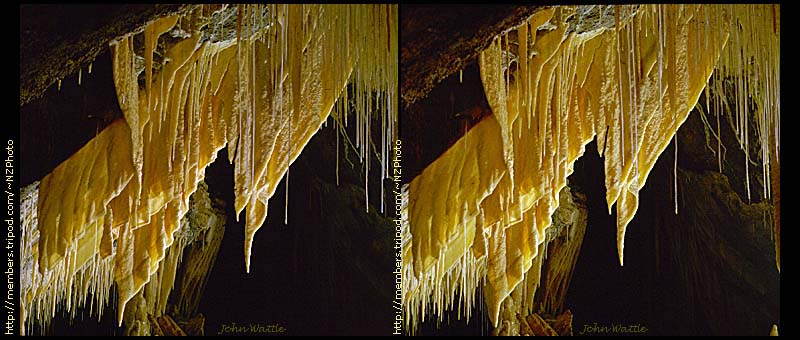
\includegraphics[width=0.9\textwidth]{IMAGES/stereoEX1.jpg}
  \end{center}
Stereo vision is among the most important human sensing methods.
\medskip
Next lecture we will talk a lot about stereo vision.
\end{frame}




% ----------------------------------------------------
\begin{frame}
\frametitle{Stereo}
In stereo we analyze two images of the same scene but obtained from
different viewpoints. Physical scene points project to corresponding
image points. \\[5mm]

\begin{center}
  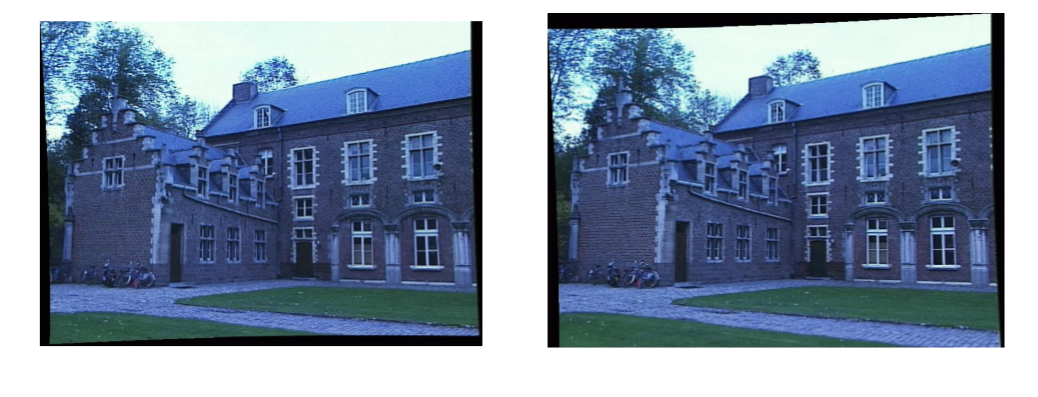
\includegraphics[width=0.9\textwidth]{IMAGES/stereo2images.png}
\end{center}

\begin{itemize}
\item How are corresponding points related ? \\[3mm]
\item May we reduce the 2-dimensional correspondence problem to 1D
  ?\\[3mm] 
\item Can we estimate relationship and is it numerically stable ?
\end{itemize}

 \end{frame}
 
 

\begin{frame}
  \frametitle{Multiple View Correspondences}
  \begin{center}
    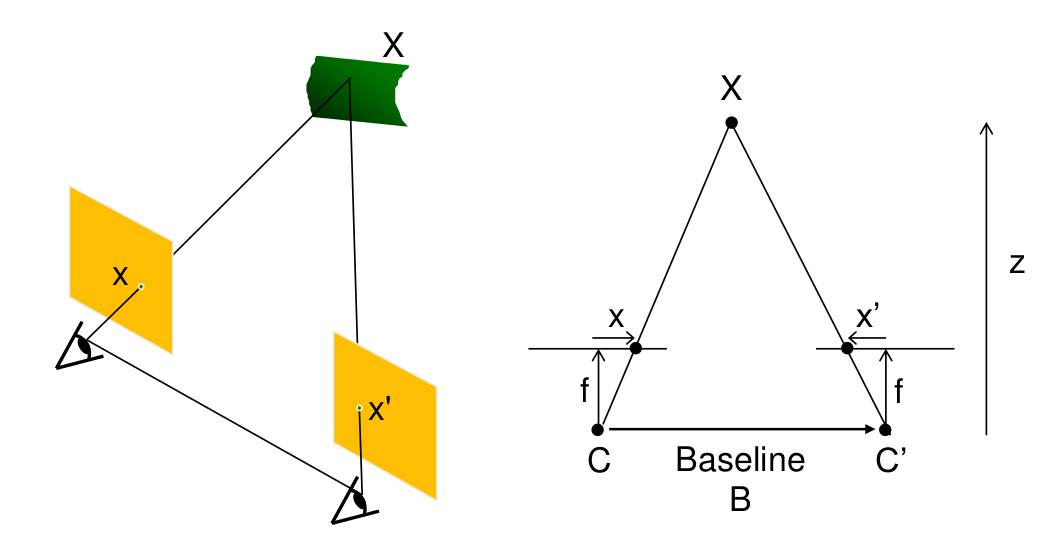
\includegraphics[width=0.9\textwidth]{FIGURES/stereo.png}
  \end{center}
  If we can recover $x'$ from $x$ we can recover depth: $z = - \frac{fB}{x'-x}$.
\end{frame}



%----------------------------------------------
\begin{frame}
\frametitle{Correspondence analysis}
Problem statement:  
{\color{blue}{Establish pairs $({\bf p_L}, {\bf p_R})$ of image 
points ${\bf p_L}$ in the left image and ${\bf p_R}$ in the
right image such that both points are projections of the same physical
scene point}}. \\[5mm]

  \begin{itemize}
  \item Correspondence analysis is the difficult part of stereo
    analysis \\[4mm]
  \item Correspondence analysis is the basic of many other
    applications, eg. stitching, geo-referencing, image
    alignment/warping etc. \\[4mm] 
  \item Most mammalians have stereo vision \\[4mm]
  \item Except for auto-focus cameras, stereo is the most widely
    applied passive  technique for 3D-measurement.
  \end{itemize}
\end{frame}





%----------------------------------------------
\begin{frame}
  \frametitle{Problems}

  \begin{minipage}{0.4\textwidth}
  \begin{itemize}
  \item Intensity in corresponding points are not equal: $E_L \neq E_R$.
  \item Many geometric properties, eg. orientation, are not preserved
    under perspective projections. 
  \item Occlusions: Things/areas visible en one image is invisible in
    the other.
  \item Double nail illusion
  \end{itemize}
  \end{minipage}
  \begin{minipage}{0.5\textwidth}
  % Show image pair with large occlusions
  % \begin{center}
  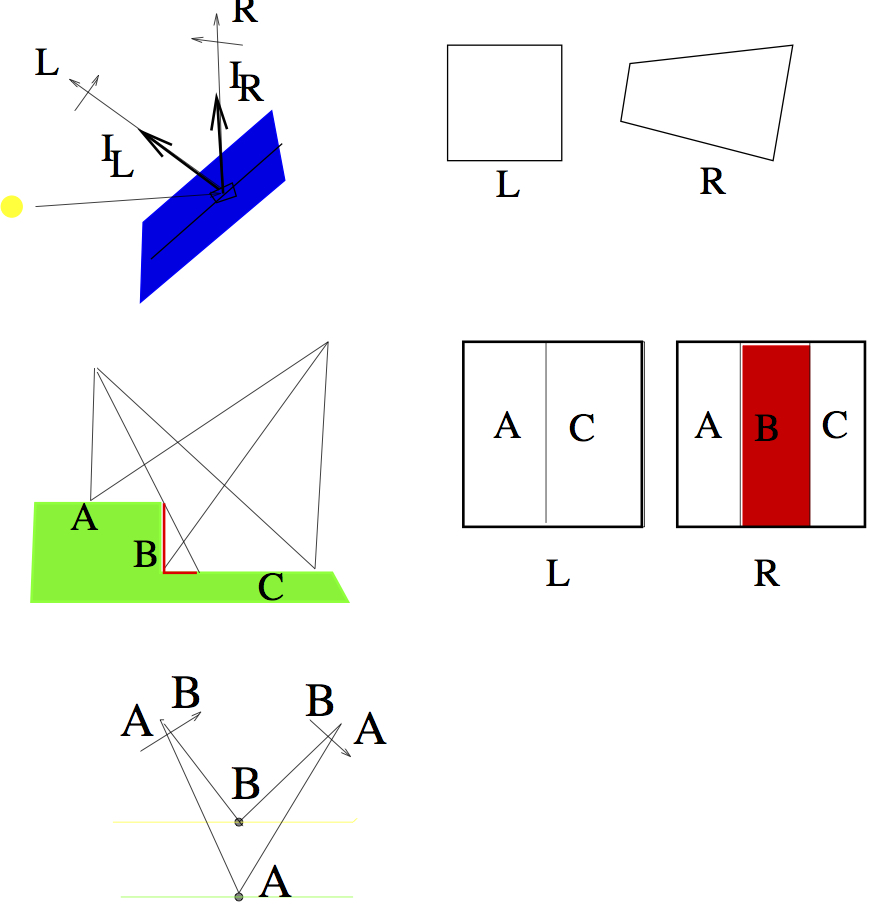
\includegraphics[width=\textwidth]{FIGURES/probilust1.jpg}
  % \end{center}
  \end{minipage}

\end{frame}





%----------------------------------------------
\begin{frame}
  \frametitle{More problems}
 \begin{itemize}
  \item Lack of texture/structure/intensity variation makes 
    makes feature matching difficult and intensity comparison
    vulnerable. 
  \item Complexity of correspondence problem: Given point in one
    image, how many possible matches exist in the other image ?
  \end{itemize}

  \begin{center}
  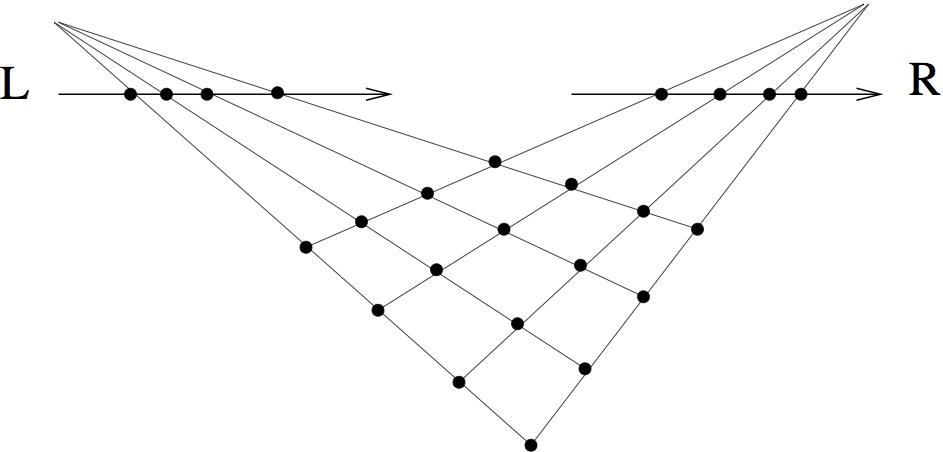
\includegraphics[width=0.8\textwidth]{FIGURES/kompleksitet.jpg}
  \end{center}

\end{frame}





%----------------------------------------------
\begin{frame}
\frametitle{Complexity}
Assume $n$ points along both epipolar lines. $N(n)$ is number
of solutions.
  \begin{center}
    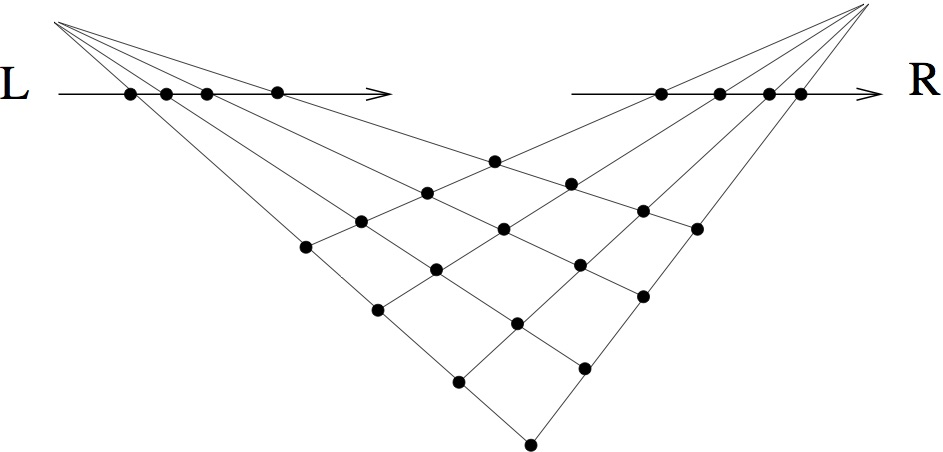
\includegraphics[width=0.4\textwidth]{IMAGES/kompleksitet.jpg}
  \end{center}
 
Without assumptions:  
$N(n) \;=\; 2^{n^2}$. 
$N(4) \;=\; 65536$ \\[2mm]

Assume that each point may match at most one other point:
$N(n) \;= \; \sum_{i = 0}^{n} \frac{(n!)^2}{(n-i)! (i!)^2}$. 
$N(4) \;=\; 204$. \\[2mm]

Assume ordering, ie. 
$x_L^1 \leq x_L^2 \; \Rightarrow \; x_R^1 \leq x_R^2$, and uniqueness:  \\
$N(n) \;=\; \frac{(2n)!}{(n!)^2}$. 
$N(4) = 70$. \\[2mm]

% Assume strong ordering: All L-points match exactly one R-point: \\
Assume all L-points match exactly one R-point: \\
$N(n) \;=\; n!$. 
$N(4) \;=\; 12$. \\[2mm]

Assume strong ordering and uniqueness: \\
$N(n) \;=\; 1$.

\end{frame}



%----------------------------------------------
\begin{frame}
  \frametitle{Simplifying assumptions}
  \begin{itemize}
  \item Intensities are similar, eg. $|E_L - E_R| \leq \theta$ or are
    spatially correlated (more later). \\[3mm]
  \item Fundamental matrix is estimated $\implies$ matching is reduced
    to 1D along epipolar lines. \\[3mm]
  \item The world consist of solid textured surfaces. Thus, the
    disparity is a single-valued function, and there exist a {\em
      unique} solution to the correspondence problem. \\[3mm]
  \item Occlusions and depth discontinuities do not exist. \\[3mm]
  \item Ordering: Corresponding points appear in the same order along
    the epipolar lines. \\[3mm]
  \item The magnitude of the disparity gradient is limited (for humans
    to about 1).    
  \end{itemize}
\end{frame}





%----------------------------------------------
\begin{frame}
\frametitle{Example: Large disparity gradient 1}

% Large disparity gradient (0.6):
\begin{center}
  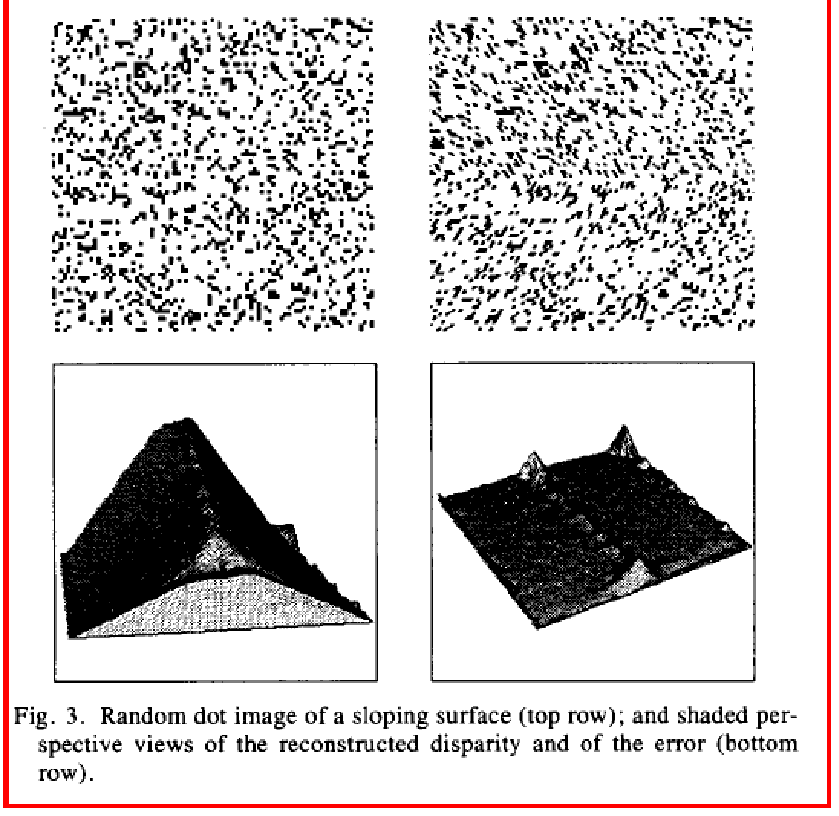
\includegraphics[width=0.6\textwidth]{IMAGES/largegradient.pdf}
\end{center}

Humans can fuse random dot stereograms with no structural information.
Image has a disparity gradient of 0.6. Humans cannot fuse images with
gradient larger than 1.
\end{frame}


%----------------------------------------------
\begin{frame}
\frametitle{Example: Large disparity gradient 2}

\begin{center}
  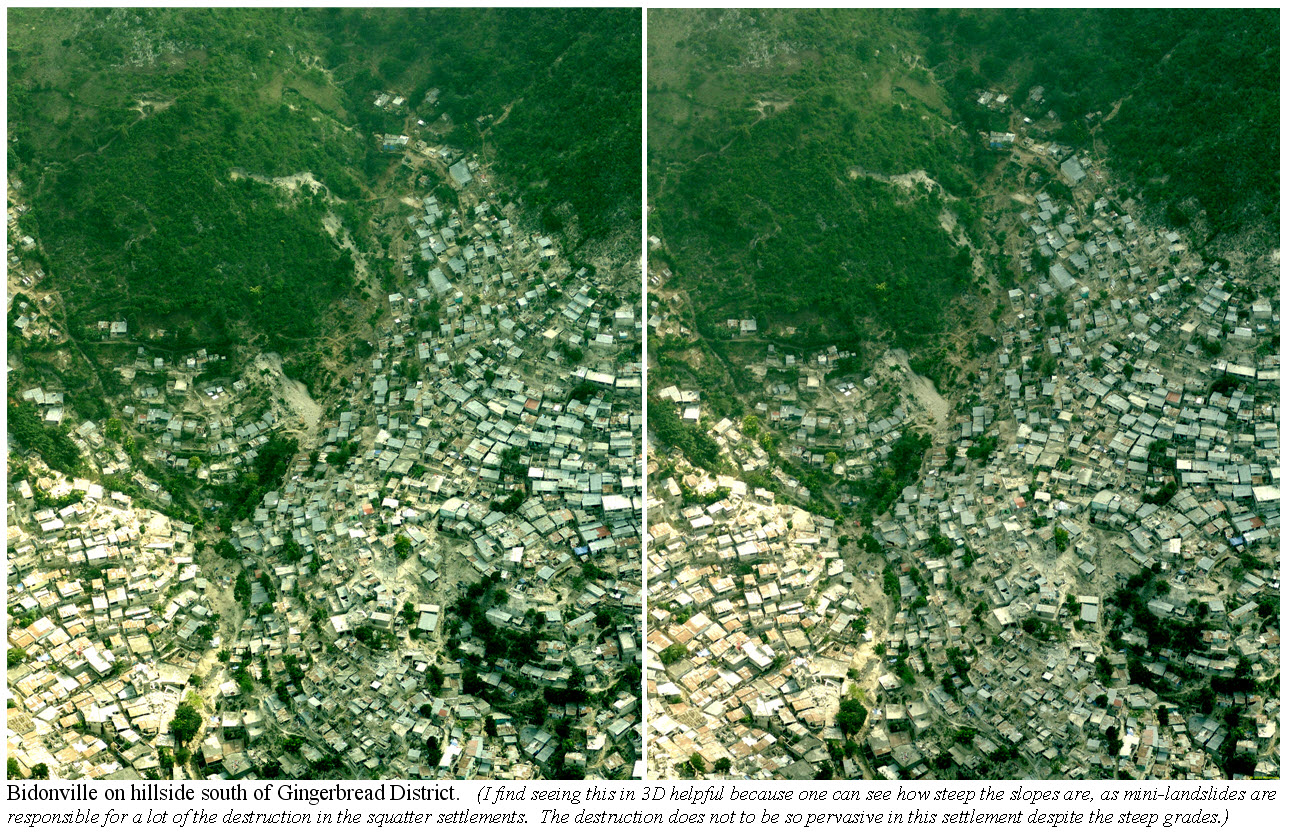
\includegraphics[width=0.9\textwidth]{IMAGES/StereoPair-of-Bidonville.jpg}
  \end{center}
\end{frame}





%----------------------------------------------
\begin{frame}
\frametitle{Example: What surface ?}

% stereo image of tree - do we have surfaces ?
  \begin{center}
  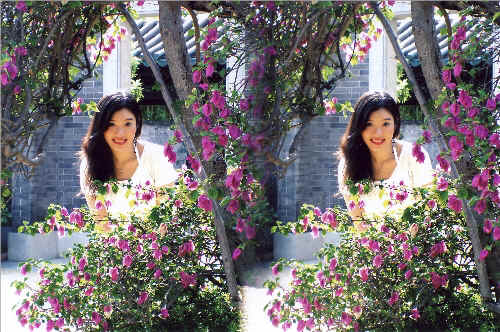
\includegraphics[width=0.9\textwidth]{IMAGES/loreo01.jpg}
  \end{center}
\end{frame}




%----------------------------------------------
\begin{frame}
  \frametitle{Correspondence analysis}
  \begin{itemize}
  \item {\color{red}{Dense intensity based methods}} may be accurate but is very
    noise sensitive and have a small capture area. Also, they may be
    computationally expensive. \\[5mm]
   \item {\color{red}{Sparse feature based methods}} is faster, more reliable, and
     have larger capture area, but results in scattered depth information.\\[3mm]
  \item {\color{blue}{Very local}} features as edge points often has a
    short descriptor, e.g. edge orientation. \\[5mm] 
  \item {\color{blue}{Less local}} features (as SIFT) is less dense, but often has a
            more expressive descriptor. \\[5mm]
  \item {\color{blue}{Large features}} (as image segments) are few and
    more easy to match, but gives less depth information. 
  \end{itemize}
\end{frame}





% ----------------------------------------------
\begin{frame}
  \frametitle{Feature based stereo}
  \begin{itemize}
  \item Detect interest (eg. SIFT) points in both images
  \item Attribute interest point with (eg. SIFT) descriptors
  \item Match the points with most similar descriptors
  \item Eliminate false matches that does not comply with the
    fundamental matrix equation
  \item Gather more matches or fit dense surface (optional)
  \end{itemize}
  \bigskip
  
  Procedure above often done coarse-to-fine to speed up and reduce blunders
\end{frame}





% ----------------------------------------------
\begin{frame}
\frametitle{Area based stereo}
  \begin{itemize}
  \item Pixelwise intensity comparison does not work. Areas, say 
    $7 \times 7$, or $13 \times 13$ are used. Larger windows implies
    better robustness, less precision and larger vulnerability to occlusions.
  \item All R-windows centered and displaced along the epipolar line
    are compared to the L-window centered at the point in question and
    the best is chosen.
  \item Typical measure: {\color{green}{Normalised cross-correlation}}
  \end{itemize}

\begin{center}
  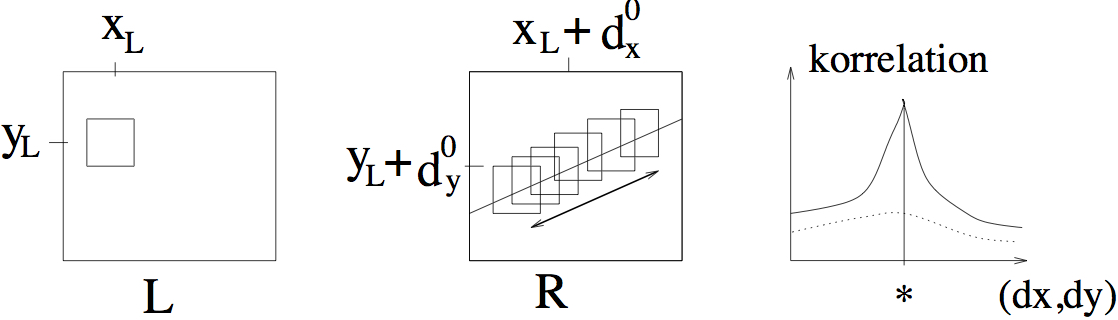
\includegraphics[width=0.9\textwidth]{FIGURES/arealstereo.jpg}
\end{center}
\end{frame}


%----------------------------------------------
\begin{frame}
  \frametitle{Disparity Map By Dense Block Matching\footnote{Slide adapted from  Derek Hoiem}}
  \begin{center}
    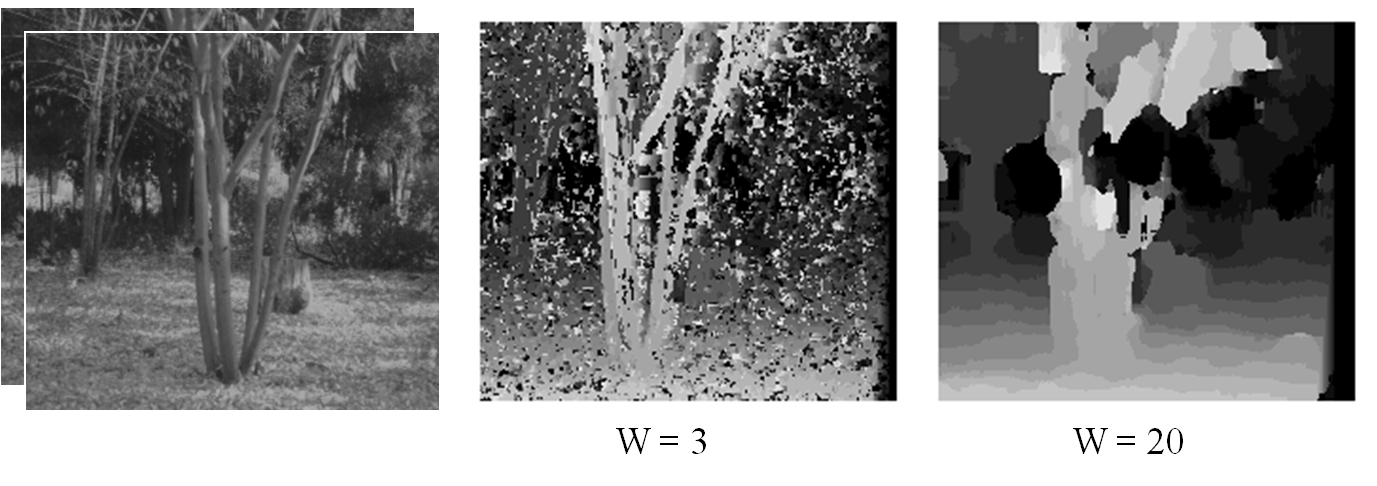
\includegraphics[width=\textwidth]{IMAGES/ddmapsblockmatch}
  \end{center}
  \begin{itemize}
  \item Window size 3: Noisy but detailed.
  \item Window size 20: smoother, but missing details.
  \end{itemize}
\end{frame}



%----------------------------------------------
\begin{frame}
\frametitle{Cross-correlation}
The cross-correlation between two continuous functions (with limited
square integral) is defined by:
\begin{displaymath}
  h(x) = (f \circ g)(x) \;\;=\;\; \int
        f^{\star}(\alpha) g(x \;+\; \alpha) d\alpha
\end{displaymath}
 
Discrete normalised 2D cross correlation is defined by:
\begin{displaymath}
  \frac{1}{n} \sum_{(x,y) \in \Omega}
  \frac{(f(x,y) - \bar{f}) \cdot  (g(x + \alpha,y + \beta) - \bar{g})}
    {\sigma_f \sigma_g}
\end{displaymath}
where $n$ is the number of pixels in $\Omega$, $\bar{f}$ is the mean
value of $f$ in $\Omega$, $\sigma_f$ is the standard deviation of $f$
within $\Omega$ (and similarly for $g$).
\medskip

Cross-correlation is used in {\color{red}{Template matching}}
where we are searching for positions in $f(x,y)$ where the
signal/image is identical/similar to the prototype $g(x,y)$.  
Such positions can be identified as the local maxima's of 
$(f \circ g)(x,y)$.
\end{frame}




%----------------------------------------------
% \begin{frame}
% Cross-correlation between an image and a prototype and the image 
% patches centered at the local maximum.  \\
%
% \begin{tabular}{l c r}
%   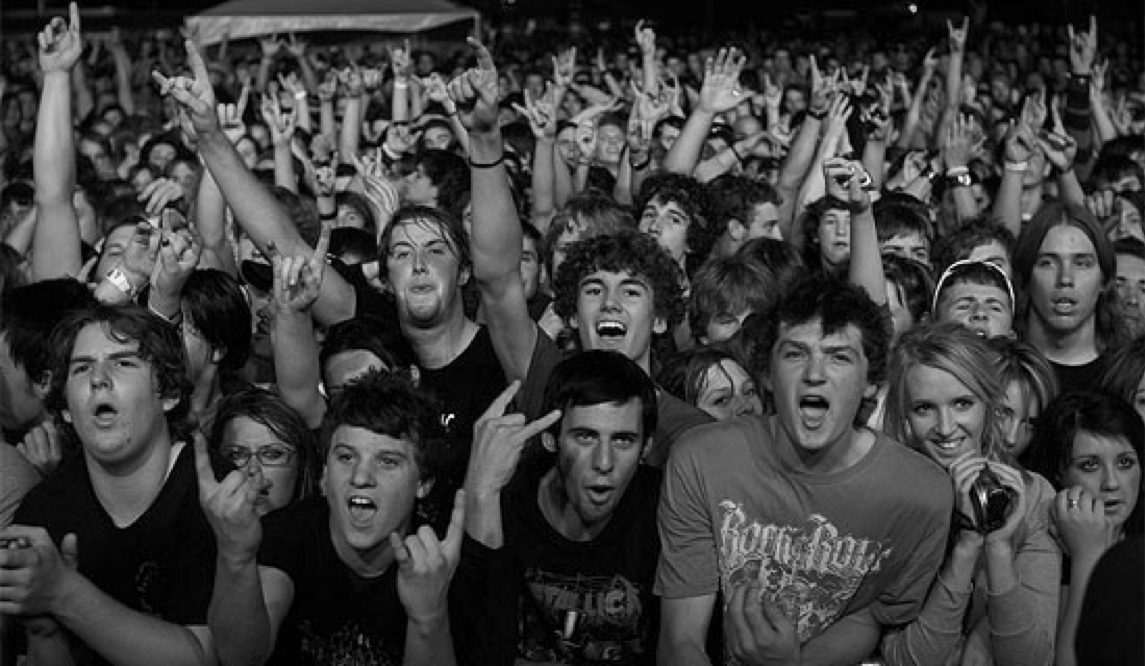
\includegraphics[width=4.8cm]{FIGURES/crowd.eps} 
%   & \hspace{2mm} & 
% %%  \begin{center}
%       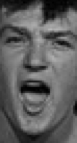
\includegraphics[width=0.35cm]{FIGURES/face.eps} \hspace{2.0cm}
% %%  \end{center}
%   \\
%    \includegraphics[width=4.8cm]{FIGURES/correlres.eps} 
%   & \hspace{2mm} & 
%    \includegraphics[width=4.8cm]{FIGURES/corrresult.eps} 
% \end{tabular}
% \end{frame}



%----------------------------------------------
\begin{frame}
 \frametitle{3-Camera stereo}

The use of 3 cameras in stereo vision, and assuming all fundamental
matrices known, makes the correspondence analysis more easy and
robust. 

\begin{center}
      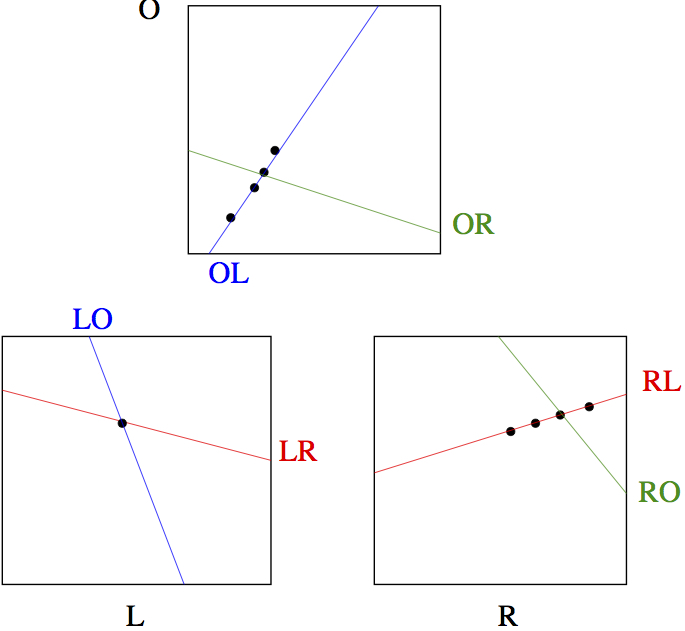
\includegraphics[width=0.6\textwidth]{FIGURES/kamera3.jpg}
\end{center}

\end{frame}



%----------------------------------------------
\begin{frame}
\frametitle{Scale-Space -repetition}
Often we don't know the size of the things we are imaging, so we have
to use both large and small filters when we analyse images. In
practice we represent each image at a number of scales. \\[6mm]

A scale-space representation is obtained by convolving the image with
Gaussian kernels of increasingly larger size.
%
% Please check previous slides for the definition and details on
% scale-space. \\[6mm] 
At small scales we only blur the images slightly to attenuate noise.
At large scale we blur heavily to ensure that only large scale
structures survive. \\[6mm]
% 
% The 2D-Gaussian filter has a number of unique properties, that makes
% it the default smoothing filter.  \\[3mm]

To save space and (in particular) time we subsample the smoothed image
versions. The result is an image pyramid.

% Often the large scale images are subsampled (according to the sampling
% theorem) to save space and to improve processing time.  
\end{frame}





%----------------------------------------------
\begin{frame}
\frametitle{Coarse-to-fine}
Pyramid-based coarse to fine approaches:
 
\begin{itemize}
  \item reduce the time complexity from $\mathcal{O}(N)$ to
    $\mathcal{O}(\log(N))$.  \\[3mm]
  \item reduce the complexity of the correspondence problem with a
    large factor (see previous slide). \\[3mm]
  \item Facilitates global operations using only local computations \\[3mm]
\end{itemize}
\bigskip

Principle: Use approximate solutions obtained at higher pyramid level
to constrain the search at lower levels.
\end{frame}


%----------------------------------------------
\begin{frame}
\frametitle{Coarse-to-fine Stereo}

\begin{minipage}{0.30\textwidth}
In practice the disparity may be large (several hundred pixels) and
have large variation (eg. from -50 to +50 pixels).  To reduce the size
of the search area we need an estimate of the disparity. 
\end{minipage}
\begin{minipage}{0.69\textwidth}
\begin{center}
  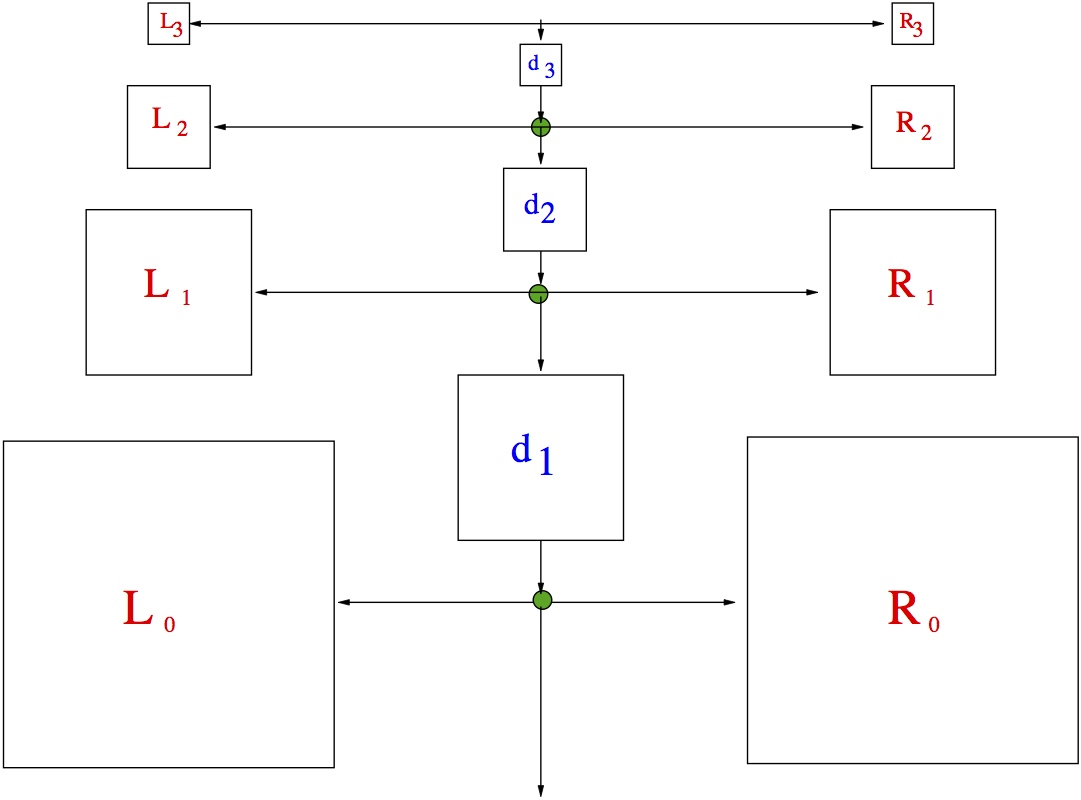
\includegraphics[width=0.75\textwidth]{FIGURES/grovfin.jpg} 
\end{center}
\end{minipage}

{\footnotesize
\begin{center}
{\color{darkgreen}{Method: Succesive smoothing and downsampling}} 
\end{center}
The total space requirement is: 
\begin{displaymath}
  1 \;+\; \frac{1}{4} \;+\; \frac{1}{16} \;+\; \cdots \;<\; \frac{4}{3}
\end{displaymath}
}
\end{frame}



%----------------------------------------------
\begin{frame}
%  \frametitle{Example}
\begin{center}
  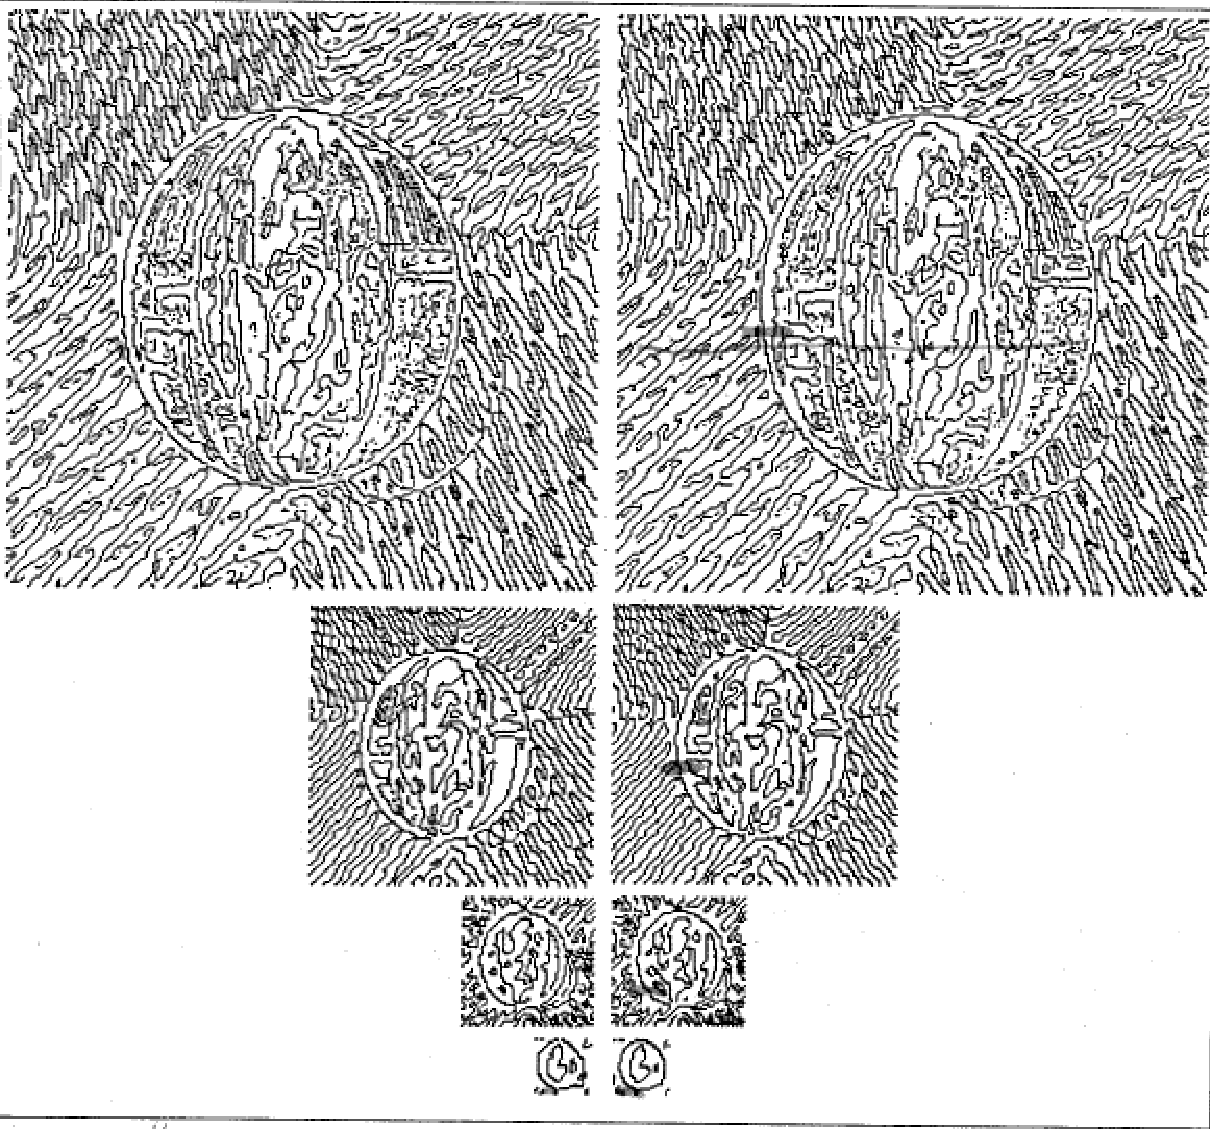
\includegraphics[width=0.8\textwidth]{IMAGES/EdgePyramidStereo2.pdf} 
\end{center}
\end{frame}



%----------------------------------------------
% \begin{frame}
%   \frametitle{Discontinuities and occlusion}
%   \begin{itemize}
%   \item It is possible to perform discontinuous regularisation, where
%     the smoothness term is disregarded when the surface is bended more
%    than some threshold. \\[3mm]
%   \item Discontinuities are accompanied by occluded areas. If any
%     point in an occluded area is matched it will be wrong. If not, the
%     surface will be reconstructed more smooth than what it should. \\[3mm]
%   \end{itemize}
%
% \begin{center}
%   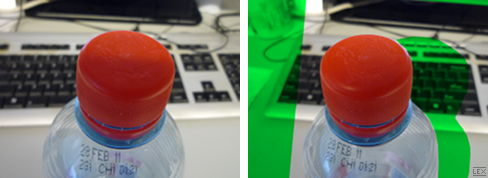
\includegraphics[width=7.0cm]{IMAGES/3d-occlusion.jpg} 
% \end{center}
% \end{frame}





%----------------------------------------------
\begin{frame}
\frametitle{Tsukuba}
{\tiny
The images in this and the next slides are from Scharstein, Szeliski:
{\em A taxonomy and Evaluation of Dense Two-Frame Stereo
  Correspondence Algorithms}, Int.Jour. of Comput.Vis. 47, 2002.
 See: \url{http://vision.middlebury.edu/stereo/data/}.
}

 \begin{center}
  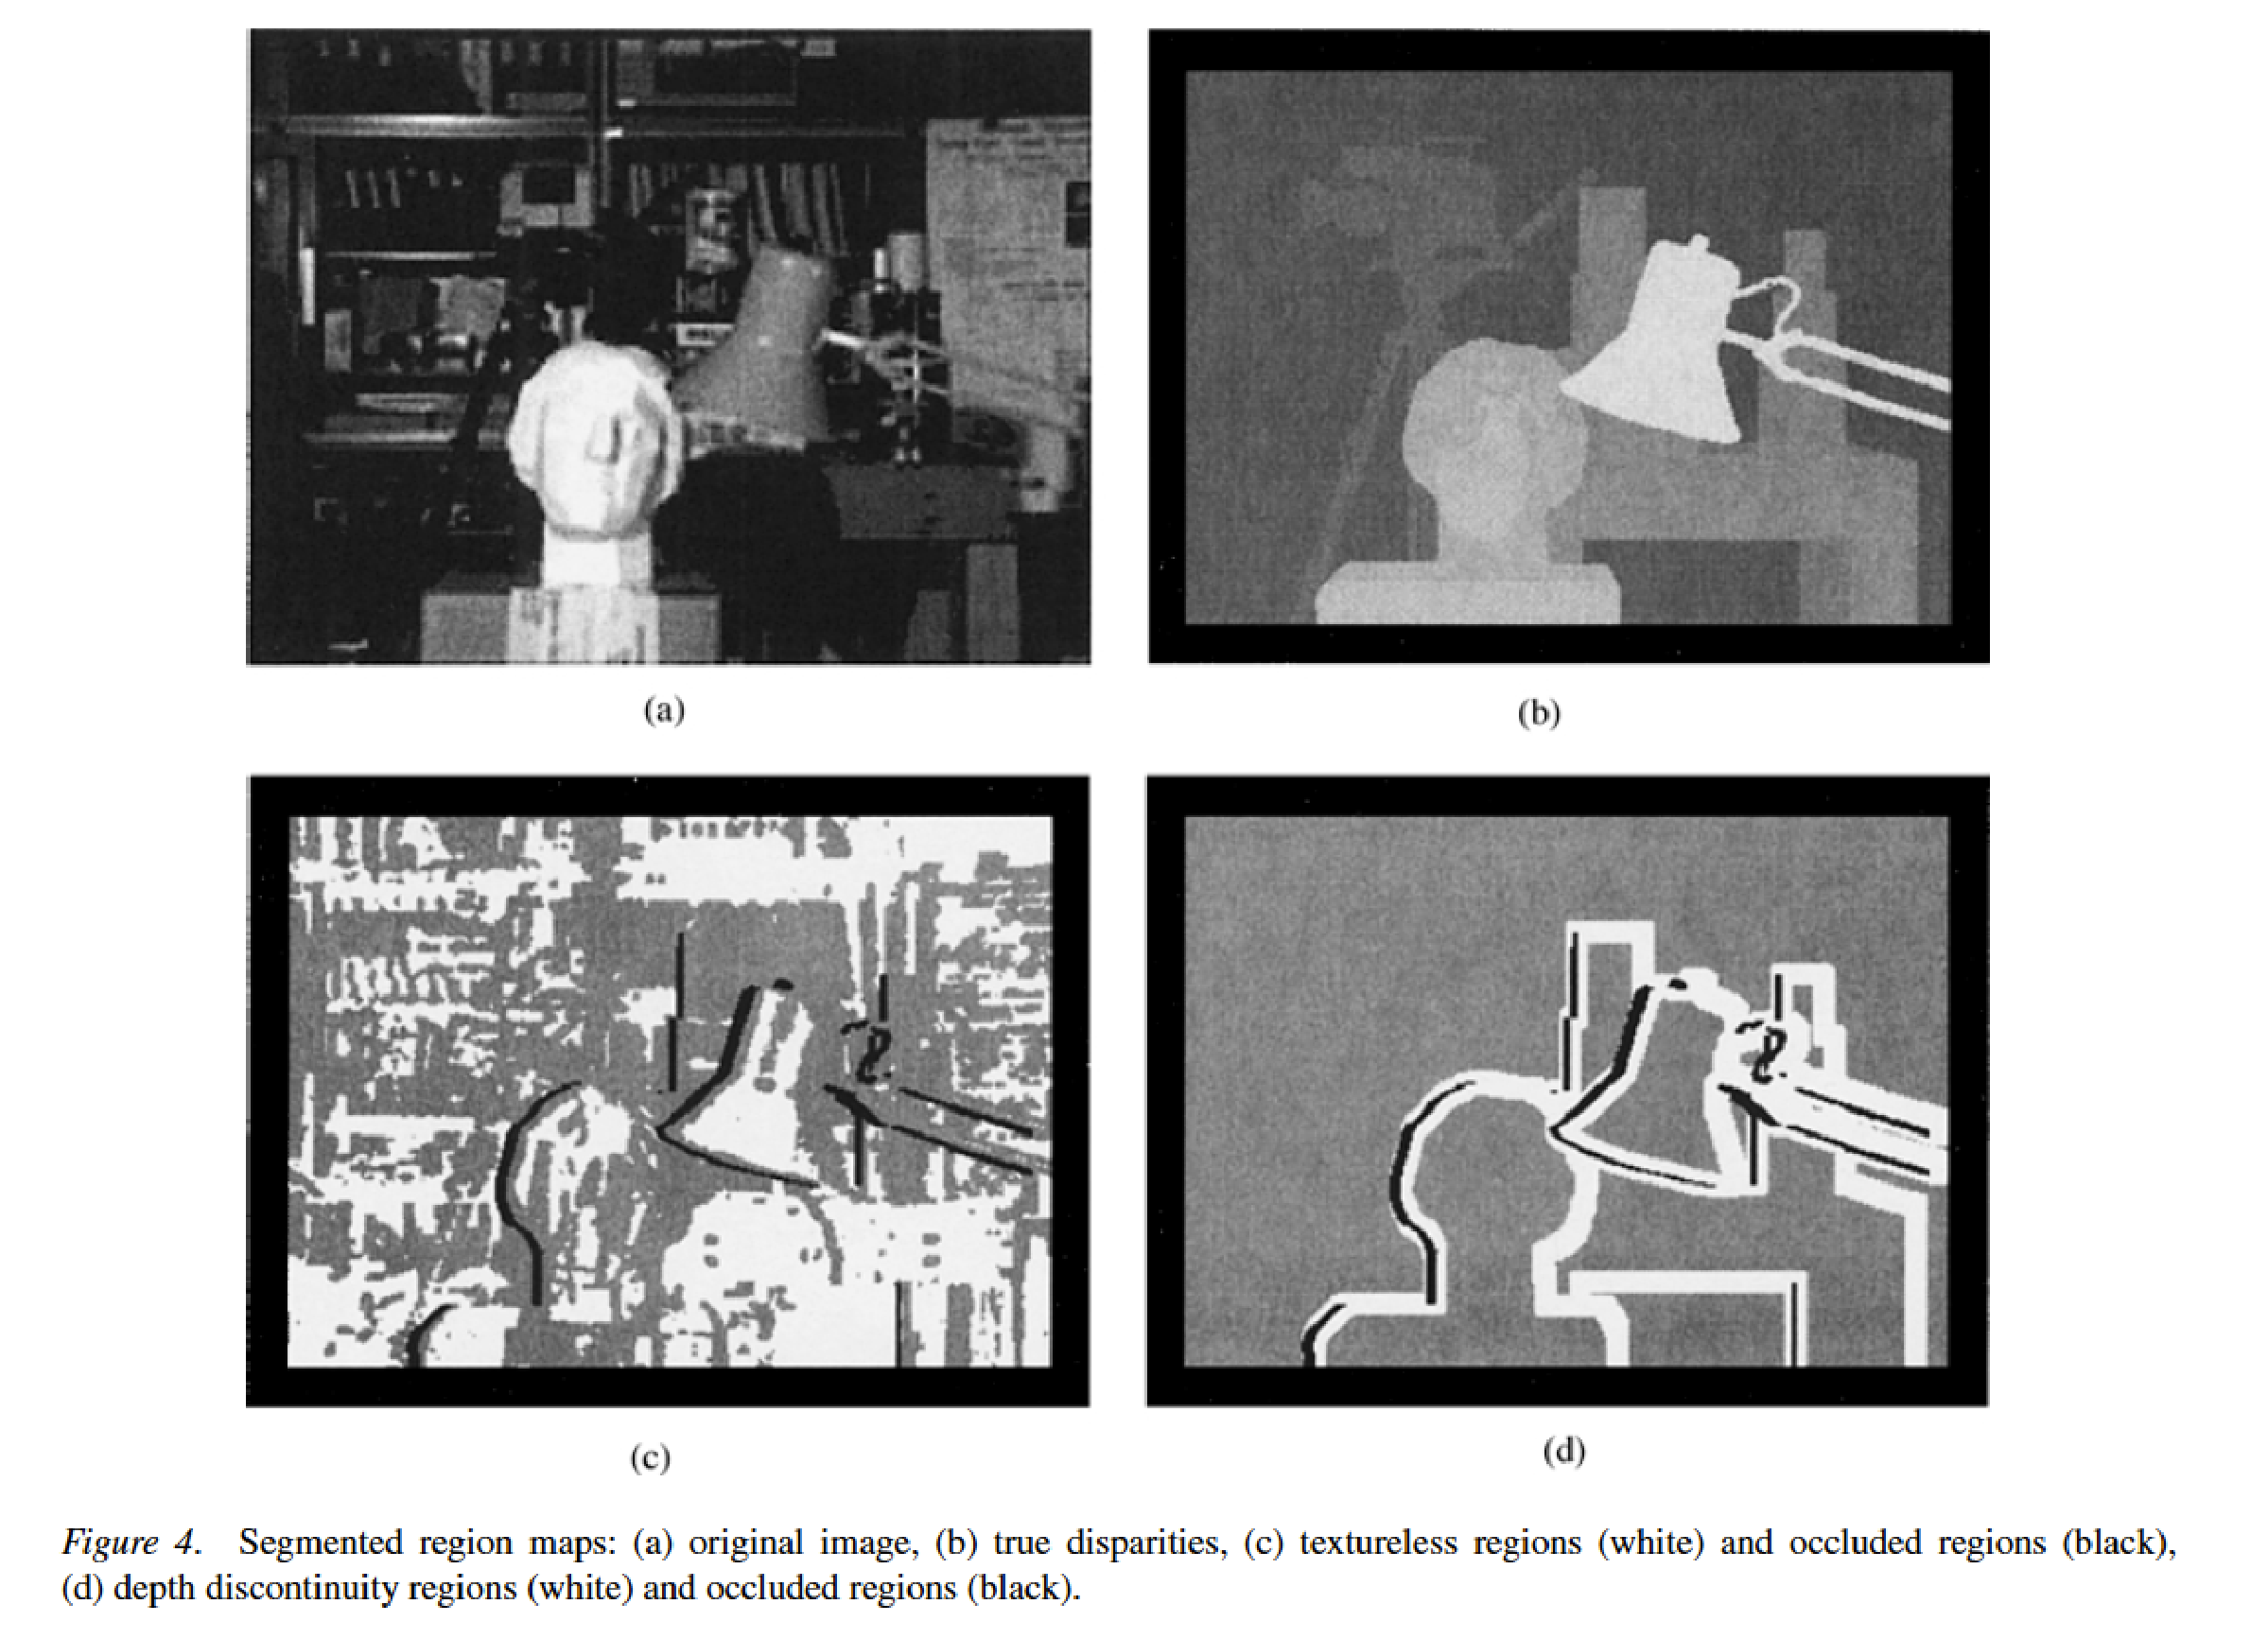
\includegraphics[width=8.0cm]{IMAGES/ImStolen.pdf} 
\end{center}
\end{frame}



%----------------------------------------------
\begin{frame}
\frametitle{Other peoples results}
 \begin{center}
  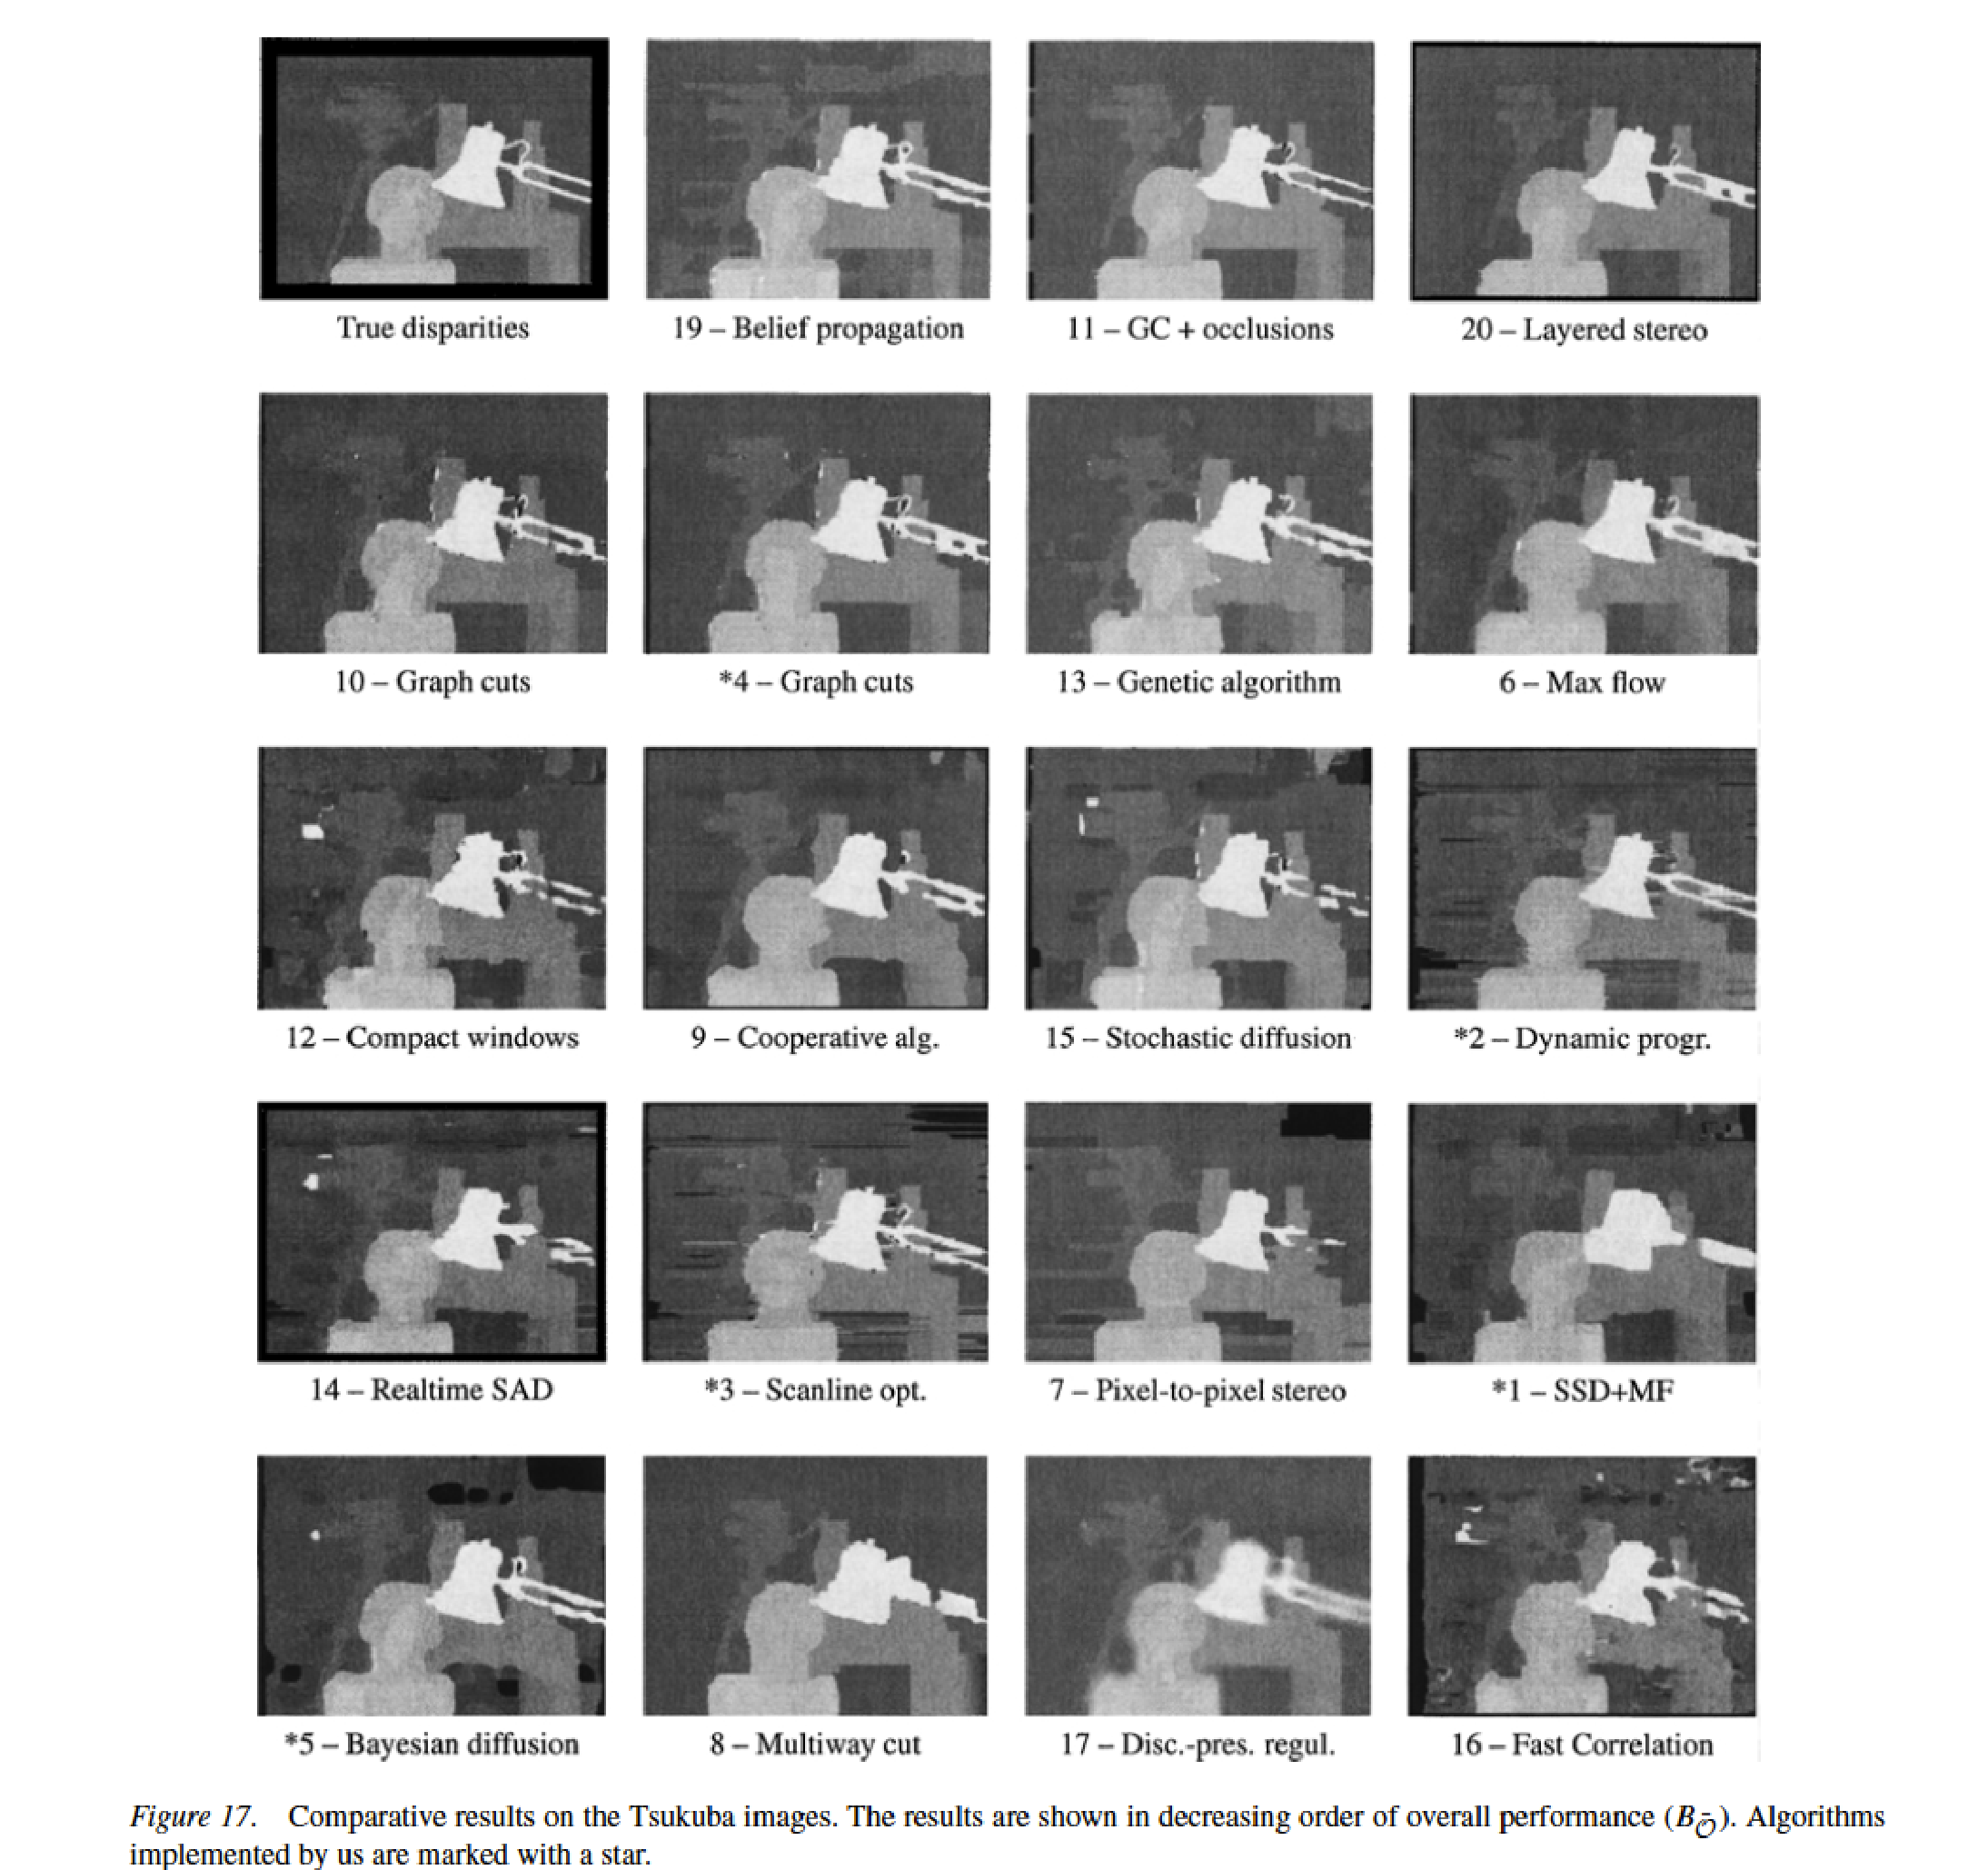
\includegraphics[width=9.0cm]{IMAGES/ImStolen2.pdf} 
\end{center}
\end{frame}





%-------------------------------------------------------------------
\begin{frame}
  \begin{center}
    {\color{blue}{\Huge QUESTIONS ?}}
  \end{center}
 \end{frame}




%---------------------------------------------
\begin{frame}
  \frametitle{Epipolar Constraints}
  \begin{center}
    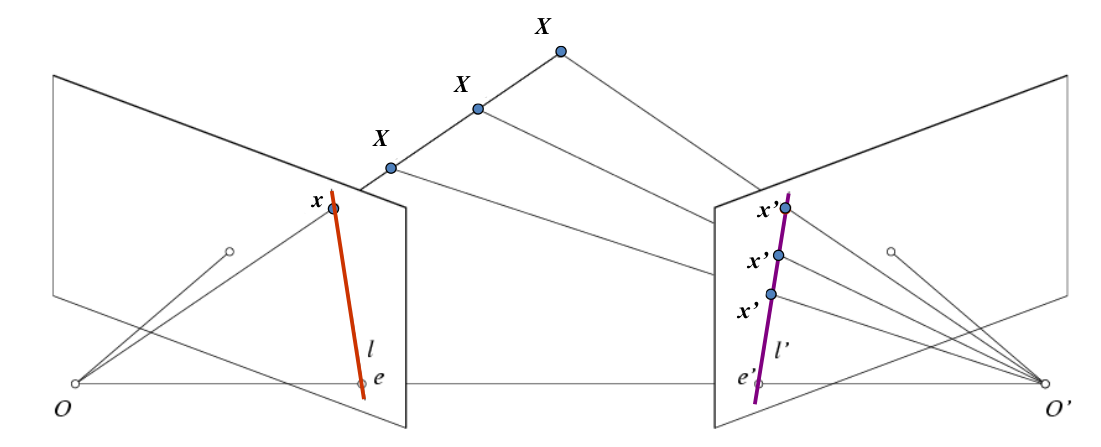
\includegraphics[width=0.9\textwidth]{FIGURES/epipolarconstraint}
  \end{center}
  \begin{itemize}
  \item  Corresponding point for $x$ must lie in corresponding line $l'$
  \item  Corresponding point for $x'$ must lie in corresponding line $l$
  \end{itemize}  
\end{frame}



%----------------------------------------------
\begin{frame}
  \frametitle{Epipolar Constraints}
  \begin{center}
    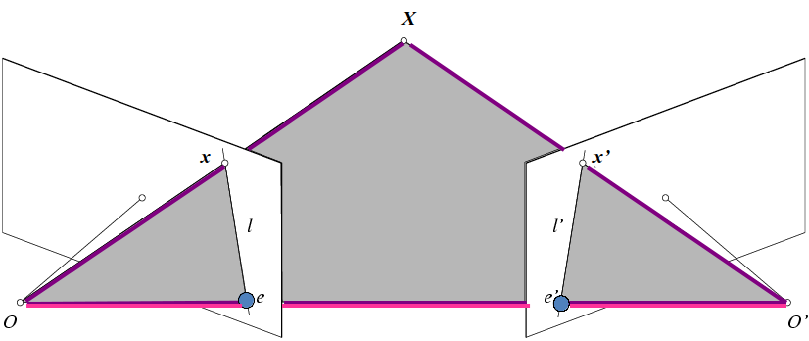
\includegraphics[width=0.9\textwidth]{FIGURES/epigeom}
  \end{center}
  \begin{itemize}
  \item  Line connecting $O$ and $O'$: \myemph{baseline}
  \item Plane through baseline and $x$ or $x'$: \myemph{Epipolar Plane}
  \item Epipoles: intersection of baseline and image planes:
    projection of the other camera center.
  \item Epipolar Lines - intersections of epipolar plane with image
    planes (always come in corresponding pairs)
  \end{itemize}  
\end{frame}


%----------------------------------------------
\begin{frame}
  \frametitle{Example: Converging cameras}
  \begin{center}
     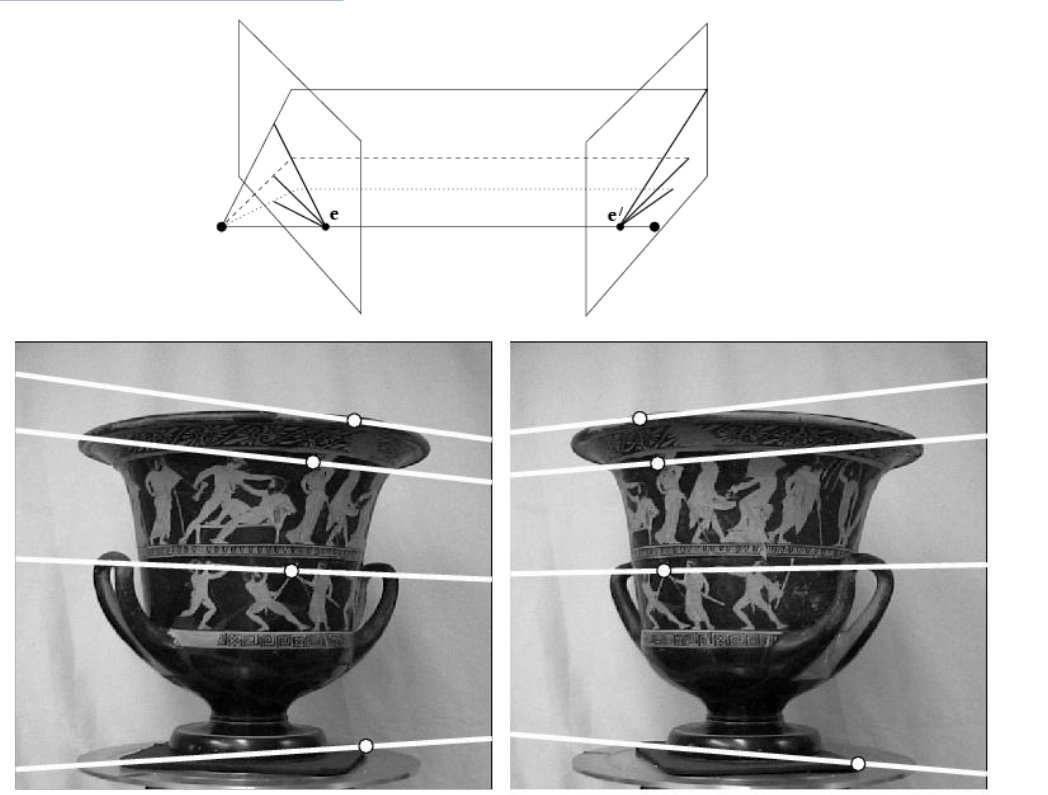
\includegraphics[width=0.9\textwidth]{FIGURES/convergecam}
  \end{center}
\end{frame}



%----------------------------------------------
% \begin{frame}
%   \frametitle{Calibrated Case}
%    \begin{center}
%     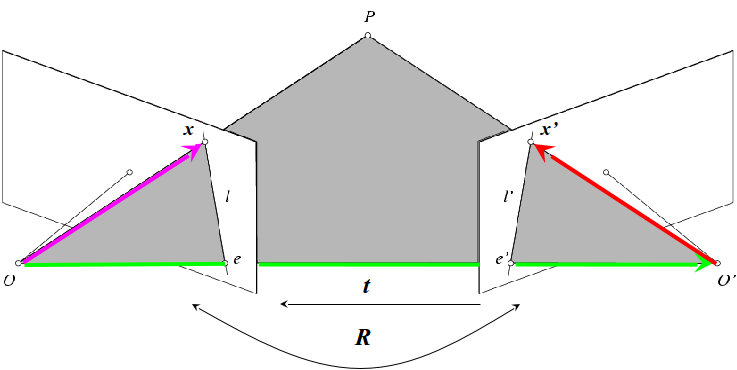
\includegraphics[width=0.65\textwidth]{FIGURES/epicalibrated}
%   \end{center}
%   Camera parameters known for the two cameras: calibration matrices $K$ and $K'$\\
% \end{frame}






%----------------------------------------------
\begin{frame}
  \frametitle{Epipolar Constraints}
  \begin{center}
    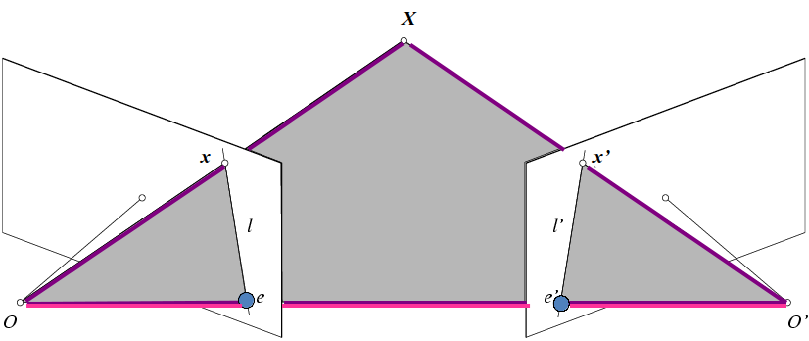
\includegraphics[width=0.9\textwidth]{FIGURES/epigeom}
  \end{center}
  \begin{itemize}
  \item  Line connecting $O$ and $O'$: \myemph{baseline}
  \item Plane through baseline and $x$ or $x'$: \myemph{Epipolar Plane}
  \item Epipoles: intersection of baseline and image planes:
    projection of the other camera center.
  \item Epipolar Lines - intersections of epipolar plane with image
    planes (always come in corresponding pairs)
  \end{itemize}  
\end{frame}



%----------------------------------------------
\begin{frame}
   \frametitle{The essential matrix $E$}
  \begin{itemize}
  \item  Let $y$ and $y'$ be 3D coordinates of the same scene point in
    the two (different) 3D-{\bf camera} coordinate systems. The two
   systems are related by a rotation and a translation. \\[3mm]
    $$y' = R(y-\bt)$$
  \item We will later show that corresponding points $y_c$ and $y'_c$
    are related by a $3 \times 3$ matrix $E$ built from $R$ and $t$  \\[3mm]
    $$
    y_c^T E y'_c = 0.
    $$
  \item $E$ is called the \myemph{essential matrix} (Longuet-Higgins
    1981).
  \end{itemize}
\end{frame}



%----------------------------------------------
\begin{frame}
   \frametitle{The fundamental matrix $F$}
  \begin{itemize}
    \item For corresponding points, the image coordinates ($x$ and
      $x'$) are related to the camera coordinates ($y$ and $y'$)
      through the calibration matrices $K$ and $K'$. Thus: 
      $$
      0 = y^T E y' = (K^{-1} x)^T E (K'^{-1} x') = 
      x^T (K^{-T} E K'^{-1} ) x' = x^T F x'
      $$
     where $x$ and $x'$ are the homogene representation of the
     corresponding points in image coordinates, and where $F$ is the
     \myemph{fundamental matrix}. \\[3mm]
   \item Given a sufficient number of corresponding image points ($x$ and $x'$),
     the fundamental matrix $F$ can be estimated.
   \item Given the internal intrinsic parameters ($K$ and $K'$) the
     essential matrix $E$ may be computed from $F$.
   \item Given $E$, the position and orientation of camera 1 vs camera
     2 (i.e., $R$ and $\bt$) can be recovered. 
   \end{itemize}
\end{frame}
 




%----------------------------------------------
\begin{frame}
  \frametitle{The Fundamental matrix}
  Ther fundamental matrix is a $3 \times 3$ matrix that relates
  corresponding points in a bilinear homogeneous equation:

  \begin{displaymath}
    \left [ x_L, \;y_L,\; 1 \right ] \; F \;
    \left [ \begin{array}{c}
              x_R \\ y_R \\ 1
            \end{array}              
          \right ] \;\; = \;\; 0 
  \end{displaymath}

  $F$ has 9 elements, but it can be shown that $\det F = 0$, so it has
  only 7 degrees of freedom (independent parameters). \\[3mm]

  Fixing either the left or right image point gives a straight line
  (the epipolar line) in the other image.
\end{frame}
 




%----------------------------------------------
\begin{frame}
   \frametitle{Calibration and reconstruction}
   \begin{itemize}
     \item Given (sufficient) image point correspondences, the
       fundamental matrix $F$ may be estimated
       using linear algebra. \\[4mm]
     \item Linear estimation of $F$   is easy, but not accurate. In
       practice a non-linear post- non-linear optimisation is needed. \\[4mm]
      \item Given $F$, the stereo correspondence problem is reduced
        to a one-dimensional search along the epipolar lines. \\[4mm]
      \item Given $F$, and the internal camera parmeters$K$ and $K'$,
        then the reconstructions of 3D points is possible (using
        linear algebra) from image point correspondences.
      \end{itemize}
      \bigskip

      If you want to know more, you must take the ATIA-course.
\end{frame}




%----------------------------------------------
\begin{frame}
\frametitle{Proof of $x_R^{\top}Ex_L = 0$}
\begin{center}
      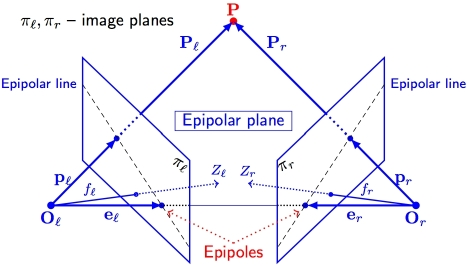
\includegraphics[width=0.7\textwidth]{IMAGES/epipolarGeom.jpg}
\end{center}
We have that the camera coordinate systems are related by:
\begin{displaymath}
   {\bf P}_R = R ( {\bf P}_L - {\bf T})
\end{displaymath}

\begin{definition}
  The coplanarity condition:  
  ${\bf P}_L$, ${\bf T}$, and 
  ${\bf P}_L - {\bf T}$ are all in the epipolar plane. Then, also
   $R^{\top}{\bf P}_R$  is within the plane.
\end{definition}
\end{frame}



%----------------------------------------------
\begin{frame}
\frametitle{The cross-product}
The cross-product between two vectors ${\bf a}$ and ${\bf b}$ is a
vector that is perpendicular to both:

\begin{displaymath}
   {\bf a} \times {\bf b} \;=\; 
   \left ( 
   \begin{array}{c}
   -a_3 b_2 + a_2 b_3 \\ a_3 b_1 - a_1 b_3 \\ -a_2 b_1 + a_1 b_2
    \end{array}
    \right )
    \;=\; S {\bf b}
\end{displaymath}
where \\[3mm]
\begin{displaymath}
   S \;=\; [a]_x \;=\; \left [
     \begin{array}{c c c}
        0    & - a_3 & a_2  \\ 
        a_3 &    0    & -a_1 \\
      -a_2 &  a_1   &  0
     \end{array}
   \right ]
\end{displaymath}

$\mbox{}$ \\[2mm]
We see that $S$ is an anti-symmetric and rank deficient matrix. $S$
has rank 2.
\end{frame}



%----------------------------------------------
\begin{frame}
\frametitle{Proof cont. 2}
Because  ${\bf P}_L$, ${\bf T}$, and ${\bf P}_L - {\bf T}$ all are in
the epipolar plane we can write:\\[3mm]

\begin{eqnarray*}
 0 & = &   ({\bf P}_L - {\bf T}) ^{\top} {\bf T} \times {\bf P}_L \\[2mm]
    & = &  (R^{\top}{\bf P}_R) ^{\top}{\bf T} \times {\bf P}_L \\[2mm]
    & = &  (R^{\top}{\bf P}_R) ^{\top} S {\bf P}_L\\[2mm]
    & = & {\bf P}_R^{\top} R S {\bf P}_L \\[2mm]
    & = & {\bf P}_R^{\top} E {\bf P}_L \\[2mm]
\end{eqnarray*}
where we have used that ${\bf P}_R = R ( {\bf P}_L - {\bf T})$ and 
$E = RS$.  
 
Since $\mbox{rank}(S) = 2$, $\mbox{rank}(E) = 2$. 
\end{frame}



%----------------------------------------------
\begin{frame}
\frametitle{The fundamental matrix equation once more}
We have now established the Essential matrix equation 
${\bf P}_R^{\top} E {\bf P}_L = 0$. To get to the fundamental matrix
equation we remember  the relation between the camera- and the image
coordinate systems:\\[3mm]

\begin{displaymath}
     K \;=\;
     \begin{pmatrix}
       \alpha & s & u_0\\
       0 & \beta & v_0\\
       0 & 0 & 1
     \end{pmatrix}
\end{displaymath}
\vspace{2mm}

Using ${\bf p}_L = K_L {\bf P}_L$ and ${\bf p}_R = K_R {\bf P}_R$ 
and defining 
\begin{displaymath}
  F \;=\; K_R^{-\top} E K_L^{-1}
\end{displaymath}
we finally get:\\[3mm]
\begin{displaymath}
   {\bf p}_R^{\top} F {\bf p}_L \;=\; 0
\end{displaymath}
\end{frame}





%----------------------------------------------
\begin{frame}
  \frametitle{Non horizontal Scan lines}
  \begin{itemize}
  \item If calibration known, the essential matrix provides epipolar
    constraints. \\[4mm] 
  \item What when cameras are in general position and calibration
    is unknown? \\[4mm]
  \item Non calibrated views: Estimate the fundamental matrix. \\[4mm] 
  \item Knowing Essential or Fundamental matrix allows (almost) for
    image rectification. 
  % \item To know more on fundamental matrices: 
  % \underline{\href{http://danielwedge.com/fmatrix}{follow the link!}}
  \end{itemize}
\end{frame}


%----------------------------------------------
\begin{frame}
  \frametitle{Projective Rectification}
  \begin{columns}
    \column{0.6\textwidth}
    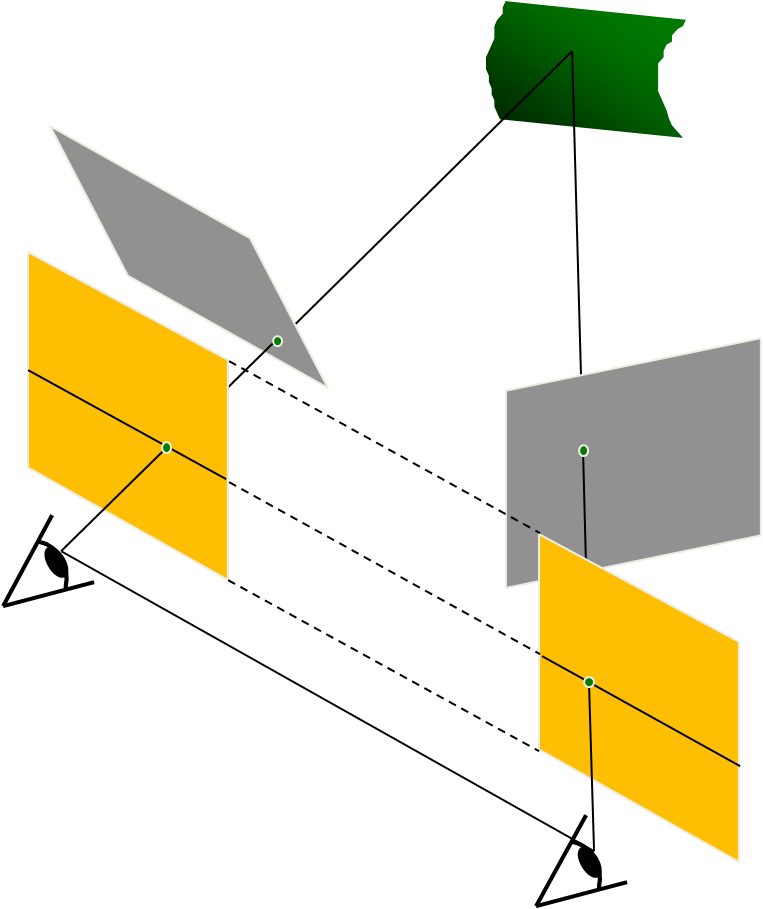
\includegraphics[width=\textwidth]{FIGURES/stereorect}
    \column{0.4\textwidth}
    \begin{itemize}
    \item Reproject onto a common plane parallel to line between camera centers
    \item Projections are homographies!
    \item Pixel motion is horizontal after reprojection.
    \item Cf Loop-Zhang, CVPR 1999 (Rectification is not easy)
    \end{itemize}
  \end{columns}
\end{frame}


%----------------------------------------------
\begin{frame}
  \frametitle{Projective Rectification example}
  \begin{center}
    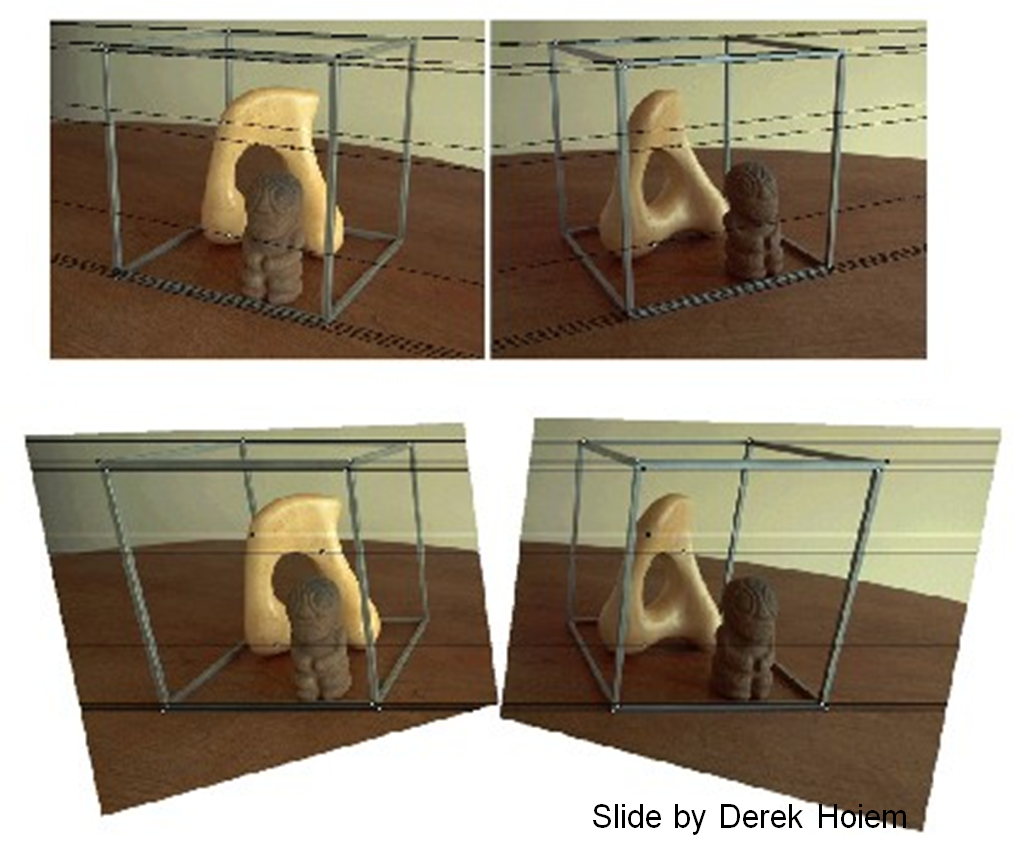
\includegraphics[width=0.8\textwidth]{IMAGES/projrectexpl}
  \end{center}
\end{frame}





% ----------------------------------------------------
 \begin{frame}
   \frametitle{Remember the Camera Matrix}
   \begin{itemize}
%   \item Combine world vs camera coordinates with
   \item Camera calibration matrix, now extended with
     Image plane transformation (axis scalings, shear, translation)
     $$
     {\bf C} = {\bf K} \left[{\bf  R}\,\, {\bf t}\right]
     $$
   \item ${\bf K}$$3\times 3$ matrix encoding the homogeneous transformations
     inside the camera. ${\bf K}$ specifies the \myemph{Intrinsic parameters}.
   \item $\left[{\bf R}\,\, {\bf t}\right]$ Concatenation of world
     coordinates rotation and origin translation to align camera and
     world coordinates.
   \end{itemize}
   $$
   \begin{bmatrix}
     x \\y \\1
   \end{bmatrix}
   =   \begin{bmatrix}
     w x \\w y \\w 
   \end{bmatrix}
   =\udesc{{\bf K}}{
     \begin{pmatrix}
       f_x & s & u_0\\
       0 & f_y & v_0\\
       0 & 0 & 1
     \end{pmatrix}}
   \udesc{\left[{\bf R}\,\, {\bf t}\right]}{
     \begin{pmatrix}
       r_{11} & r_{12} & r_{13} & t_x\\
       r_{21} & r_{22} & r_{23} & t_y\\
       r_{31} & r_{32} & r_{33} & t_z\\
     \end{pmatrix}}
   \begin{pmatrix}
     X\\Y\\Z\\1
   \end{pmatrix}
   $$
 \end{frame}


 
%----------------------------------------------
\begin{frame}
\frametitle{Given {\bf M}, how can we triangulate ?}
Let ${\bf m}^i$ be the $i$'th row of the camera matrix and
$U = (X, Y, Z, 1)^{\top}$. Then:

\begin{displaymath}
   w
   \begin{bmatrix}
     x\\y\\1
   \end{bmatrix}
   =
     \begin{pmatrix}
       {\bf m}^1 \\
       {\bf m}^2 \\
       {\bf m}^3 \\
     \end{pmatrix}
   \begin{pmatrix}
     X\\Y\\Z\\1
   \end{pmatrix}
   =
     \begin{pmatrix}
       {\bf m}^1 U \\
       {\bf m}^2 U \\
       {\bf m}^3 U \\
     \end{pmatrix}
\end{displaymath}

We will later se how we may estimate the parameters of the camera
matrix and use this to compute 3D structure (depth) from point
correspondences. 
\end{frame}


%----------------------------------------------
\begin{frame}
\frametitle{Linear triangulation for 2 calibrated cameras}
Let $U = (X, Y, Z, 1)^{\top}$.  For the first coordinate in the left camera we have:
\begin{displaymath}
 x^L  = \frac{{\bf m}_L^1U}{{\bf m}_L^3U}
\end{displaymath}
and similar for the $y$-coordinate and the right camera.  Multiplying
by the denominator we get:
\begin{eqnarray*}
   {\bf m}_L^3 x_L  U & = & {\bf m}_L^1 U \\
   {\bf m}_L^3 y_L  U & = & {\bf m}_L^2 U \\
   {\bf m}_R^3 x_R U & = & {\bf m}_R^1 U \\
   {\bf m}_R^3 y_R U & = & {\bf m}_R^2 U 
\end{eqnarray*}
Subtracting the right side and putting $U$ outside a parentesis we get
the homogeneous equation $A U = 0$, where:
\begin{displaymath}
  A  = \left (
    \begin{array}{c}
   {\bf m}_L^3 x_L   - {\bf m}_L^1 \\
   {\bf m}_L^3 y_L   - {\bf m}_L^2 \\
   {\bf m}_R^3 x_R  - {\bf m}_R^1 \\
   {\bf m}_R^3 y_R  - {\bf m}_R^2 
      \end{array}
    \right )
\end{displaymath}
\end{frame}






%-------------------------------------------------------------------
\begin{frame}
  \begin{center}
    {\color{blue}{\Huge QUESTIONS ?}}
  \end{center}
 \end{frame}







% ============================================
%  Stitching (new)
%  ----------------------------------------------


\begin{frame}
\frametitle{Stitching}
In stitching, or panorama making, several images are combined into one
larger image. 

\begin{center}
    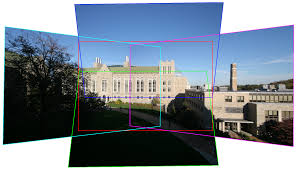
\includegraphics[width=0.64\textwidth]{IMAGES/stitching.jpg}
\end{center}

A standard transformation technique is to map the images through
homographies. However, this requires that the transformed scene
surface is planar.  Obviously this often is not the case. 
 
\end{frame}





%----------------------------------------------
\begin{frame}
\frametitle{The geometric transformation between \\ 
  two images of a planar scene}
  \begin{itemize}
   \item The perspective projection of a planar scene surface is a
     transformation $(X,Y,Z) \longrightarrow (x,y)$ called 
     an \myemph{homography}:
     $$
  \begin{bmatrix}
       w x\\w y\\w
     \end{bmatrix}
     =
     \begin{pmatrix}
       h_{11} & h_{12} & h_{13} \\
       h_{21} & h_{22} & h_{23} \\
       h_{31} & h_{32} & h_{33} 
     \end{pmatrix}
     \begin{bmatrix}
       X\\Y\\Z\\
     \end{bmatrix}
     =
     H \cdot {\bf X}
     $$
   \item The transformation between two images of a planar surface is
     an homography. 
  \item Homographies conserves straight lines, but not parallelism. 
  \item Two parallel lines intersect at infinity: after an homography
    they may intersect at finite distance. 
  \end{itemize}
\end{frame}



%----------------------------------------------
\begin{frame}
  \frametitle{Homographies}
  An homography can accurately describe the stitching of images of a
  planar scene.  Non-planar scenes cannot be stitched correctly using
  homographies. 

  \begin{center}
    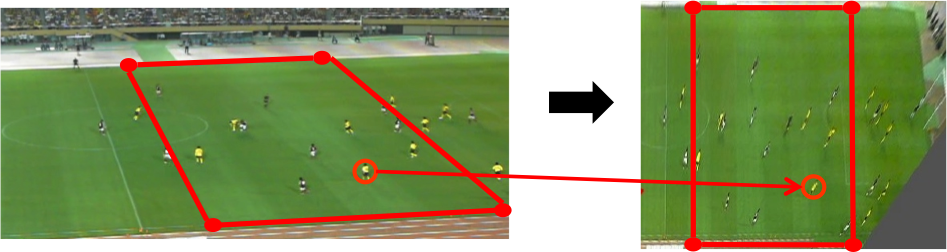
\includegraphics[width=0.85\textwidth]{IMAGES/soccer_homography.png}
  \vspace{4mm}
    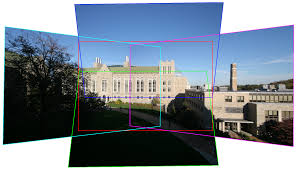
\includegraphics[width=0.6\textwidth]{IMAGES/stitching.jpg}
  \end{center}
\end{frame}



%----------------------------------------------
\begin{frame}
\frametitle{Homography estimation 1}
Let ${\bf x}$ and ${\bf x'}$ be corresponding points in homogeneous
coordinates. \\[3mm]
If ${\bf x'} = H {\bf x}$  then  ${\bf x'} \times H {\bf x} = {\bf 0}$ 
(the vectors have the same direction but may have different magnitude). \\[4mm] 

Write out the definition of the cross product and isolate the
unknown 9 elements. For compactness use 
$h = ({\bf h}_1^{\top}, {\bf h}_2^{\top}, {\bf h}_3^{\top})^{\top}$: \\[3mm]

\begin{displaymath}
\left [ 
\begin{array}{c c c}
{\bf 0}^{\top} & - {\bf x}_i^{\top} & y' {\bf x}_i^{\top} \\
{\bf x}_i^{\top} & {\bf 0}^{\top} & -x'_i {\bf x}_i^{\top} \\
 - y'_i {\bf x}_i^{\top} & x'_i {\bf x}_i^{\top} & {\bf 0}^{\top} 
\end{array} \right ]
\;
\left [ 
\begin{array}{c}
{\bf h}_1 \\ {\bf h}_2 \\ {\bf h}_3 
\end{array} 
\right ]
\;\; = \;\;
\left [ 
\begin{array}{c}
0 \\ 0 \\ 0 
\end{array} 
\right ]
\end{displaymath}
\vspace{3mm}

The last equation may be ignored because it is linearly dependent.
\end{frame}



%----------------------------------------------
\begin{frame}
\frametitle{Homography estimation 2}

In detail the nine parameters are found as the last column of the
matrix $V$ in a SVD-decomposition $A = U D V^{\top}$ of $A$, where:  \\[3mm]
\begin{displaymath}
 A {\bf h} \;=\; \left [
   \begin{array}{ccccccccc}
       0 & 0 & 0 & -x_L^1  & -y_L^1  & -1 &  x_L^1 x_R^1 &  y_L^1 x_R^1 &  x_R^1 \\
       x_L^1  & y_L^1  & 1 & 0 & 0 & 0 & - x_L^1 y_R^1 & - y_L^1 y_R^1 & - y_R^1 \\
       \vdots & \vdots & \vdots & \vdots & \vdots & \vdots &  \vdots & \vdots \\
       0 & 0 & 0 & -x_L^n  & -y_L^n  & -1 &  x_L^n x_R^n &  y_L^n x_R^n &  x_R^n \\
       x_L^n  & y_L^n  & 1 & 0 & 0 & 0 & - x_L^n y_R^n & - y_L^n y_R^n & - y_R^n \\
%   
%     x_L^n  & y_L^n  & 1 & 0 & 0 & 0 & - x_L^n x_R^n & - y_L^n x_R^n & - x_R^n \\
%     0 & 0 & 0 & x_L^n  & y_L^n  & 1 & - x_L^n y_R^n & - y_L^n y_R^n & - y_R^n \\
   \end{array}
   \right ]
    {\bf h} \;\;=\;\; {\bf 0} 
\end{displaymath}

\end{frame}





% ----------------------------------------------------
 \begin{frame}
   \frametitle{Understanding homographies}
   Since a homography $H$ can be determined up to scale only we may
   normalize to make $h_{33} = 1$:
   \begin{displaymath}
     \begin{pmatrix}
       h_{11} & h_{12} & h_{13} \\
       h_{21} & h_{22} & h_{23} \\
       h_{31} & h_{32} & 1
     \end{pmatrix}
     \end{displaymath}
     \medskip
     
     \begin{itemize}
     \item The two elements in the last colums determines translation
     \item The two elements in the last row determins perspective distortion 
     \item The four upper left elements determine rotation and scaling
     \end{itemize}
\end{frame}







%----------------------------------------------
% \begin{frame}
% \frametitle{Stitching techniques}
% Another approach is to divide the resulting image in patches and apply
% homographies to each. This obviously requires a constraint that
% transformations from neighboring patches agree. This ends up in a
% global optimization for the local homographies, but under
% regularization of a set of compatibility constraints.
%
% \begin{center}
%    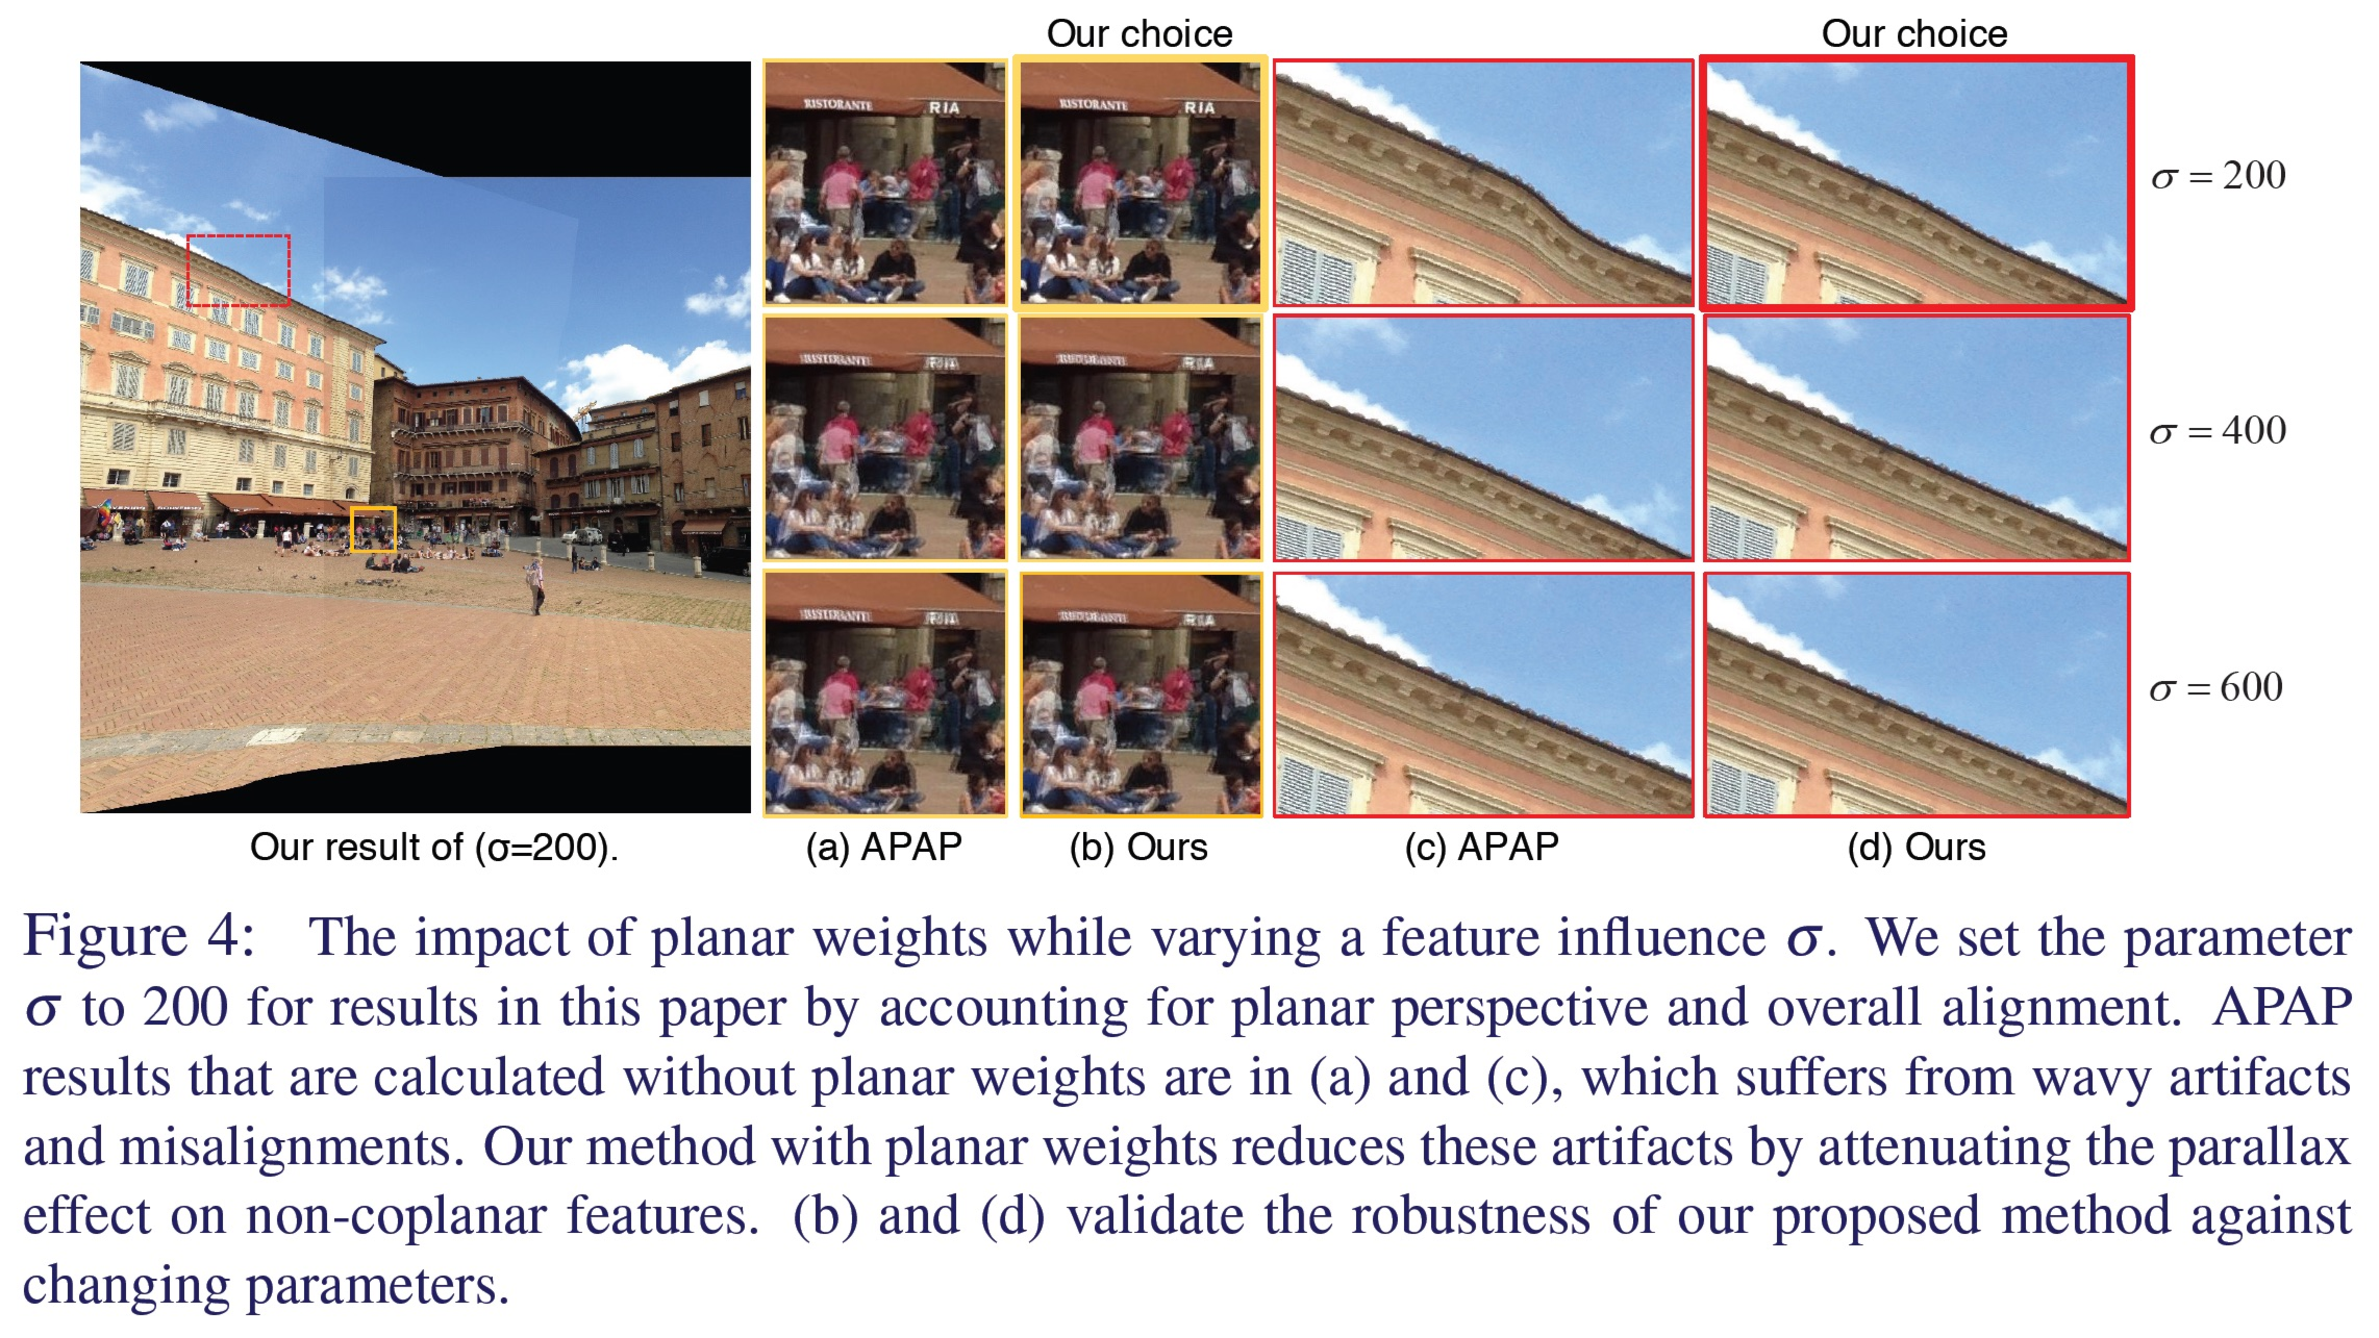
\includegraphics[width=0.80\textwidth]{IMAGES/StitchingPatches.pdf}
% \end{center}
%
% Check: {\em Szeliski: Computer Vision: Algorithms and Applications} available at: \url{http://sceliski.org/Book/}. 
% \end{frame}


%----------------------------------------------
% \begin{frame}
% \frametitle{Blending}
% When stitching hole images a general observation is that both
% intensity and color does not match, making the transition
% visible.\\[3mm]  
%
% To limit the effect a band of pixels in both images along the seam
% lines are changed gradually from the RGB-statistics on one side
% towards the statistics on the other side.
%
% \begin{center}
%      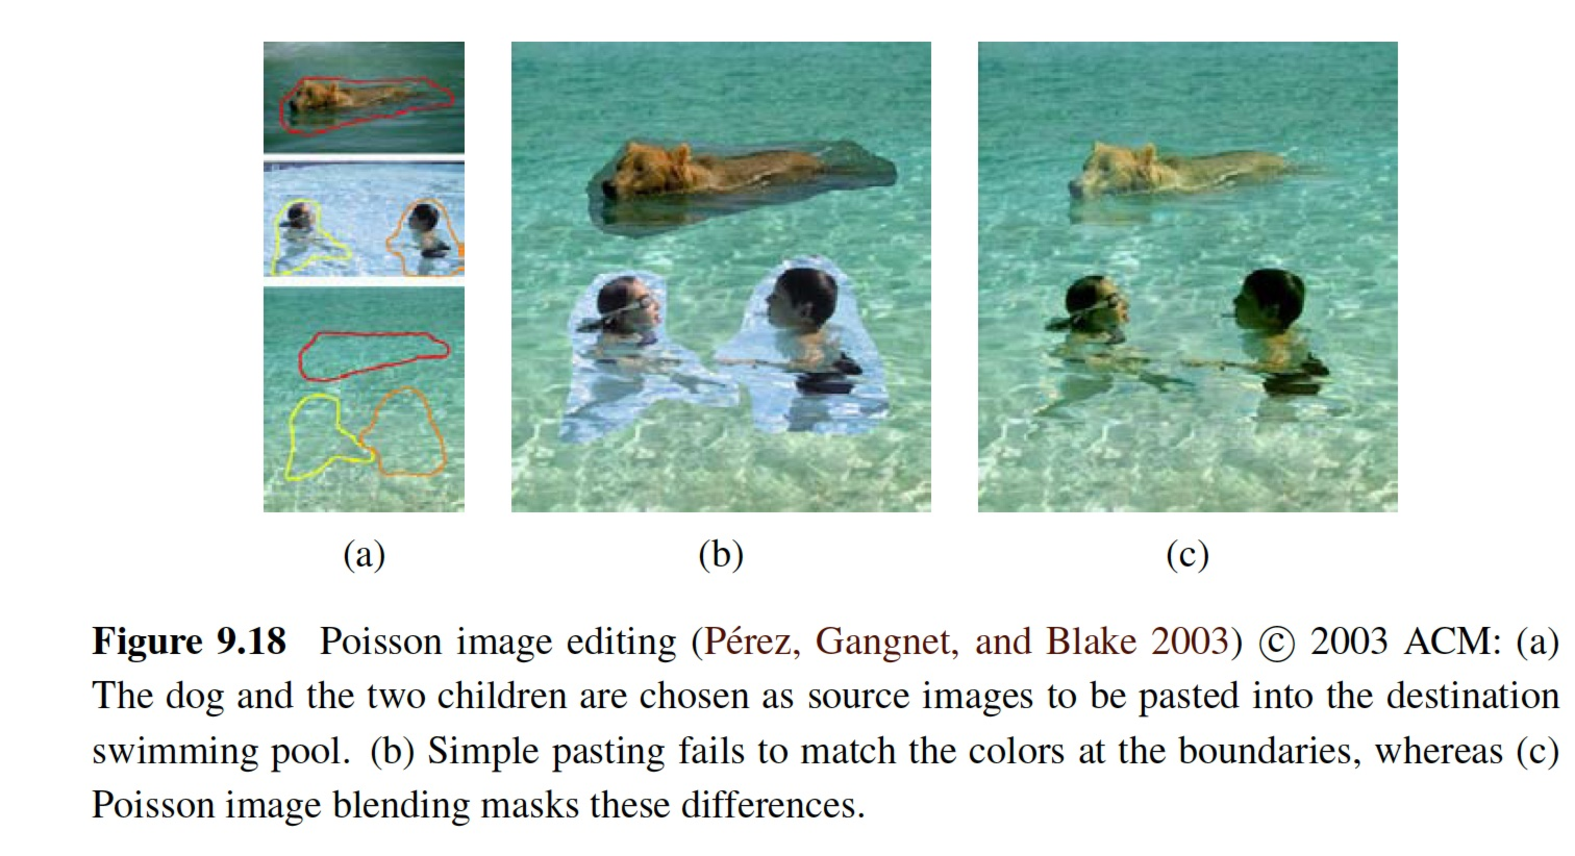
\includegraphics[width=0.88\textwidth]{IMAGES/Szeliski_blending.pdf}
% \end{center}
% \end{frame}


%----------------------------------------------
% \begin{frame}
% \frametitle{Seam lines}
% Images need not be stitched together along their border.  Significant
% visual improvement is possible by selecting the (not necessarily
% straight) seam lines. \\[4mm]
%
% A seam line is a connected set of pixels in the common coordinate
% system for two images defining where the images are glued together.
% Two principles may be used to define the seam lines: \\[4mm]
%
% \begin{itemize}
% \item The lines is chosen to minimize the color difference between the
%   two images along the line. This may be translated into a dynamic
%   programming exercise. \\[3mm]
% \item The lines are chosen to best fit the image edges where intensity
%   and color changes mostly and errors are less visible.
% \end{itemize}
% \end{frame}



%----------------------------------------------
\begin{frame}
\frametitle{Stitching example with seam-lines}
\begin{center}
    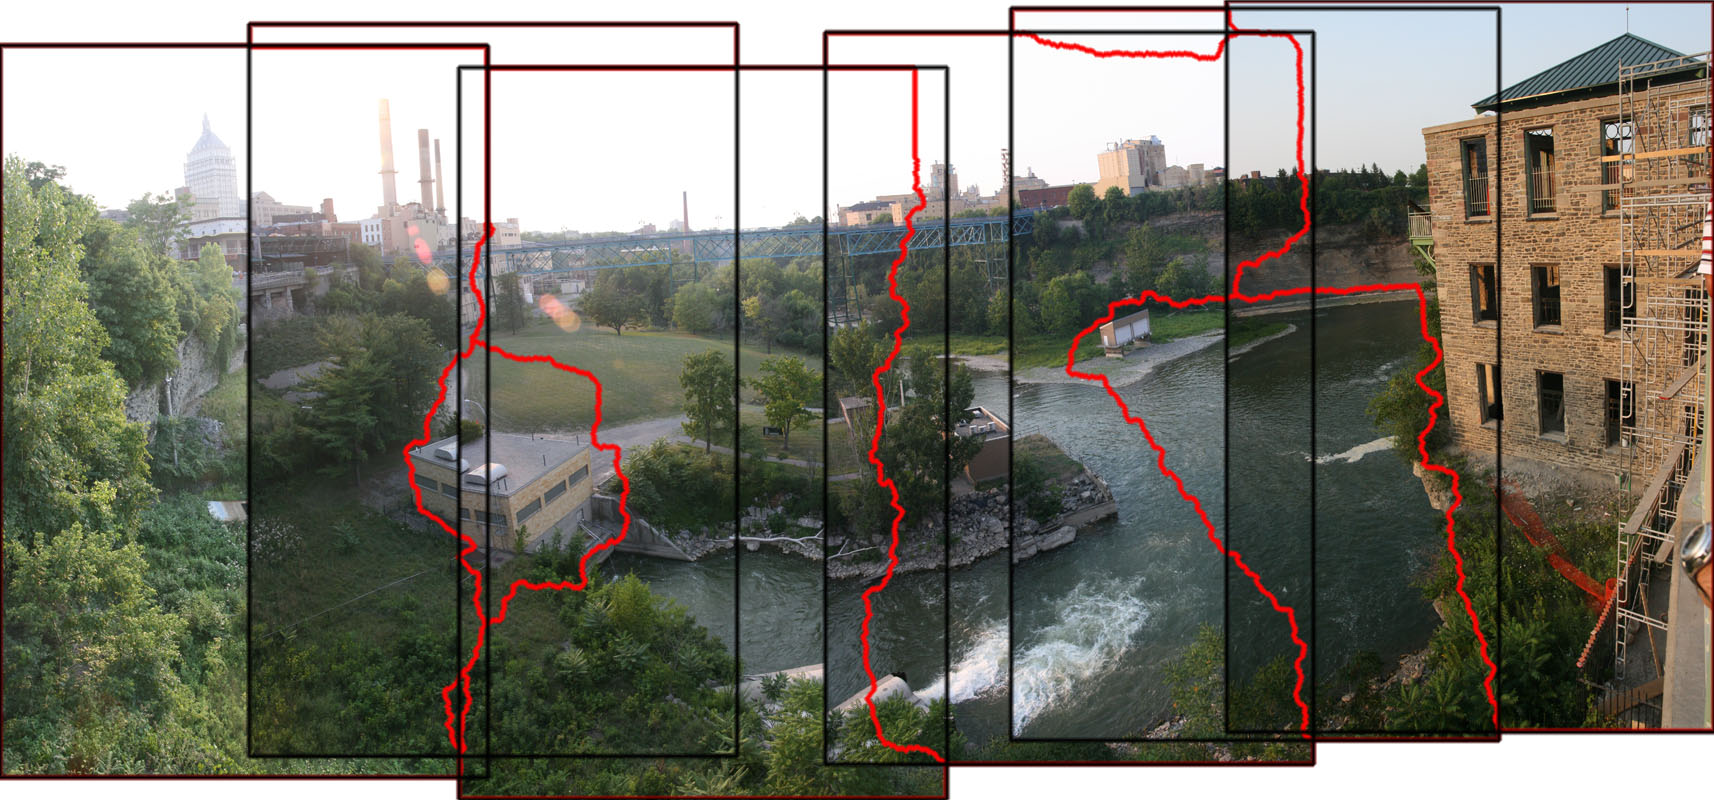
\includegraphics[width=0.99\textwidth]{IMAGES/Rochester_seamlines.jpg}
  \end{center}
 {\small (from Wikipedia)}
\end{frame}




%-------------------------------------------------------------------
\begin{frame}
  \begin{center}
    {\color{blue}{\Huge QUESTIONS ?}}
  \end{center}
 \end{frame}




%----------------------------------------------
\begin{frame}
  \begin{center}
    
\includegraphics[width=\textwidth]{IMAGES/tired}
 \end{center}
\end{frame}



\end{document}


